% NOTE: Use latexmk instead of arara
% latexmk -pvc slides.tex # Watches and compiles on each change.
% latexmk -c slides.tex   # Clean the temporal files.

%% arara: pdflatex
%% arara: bibtex
%% arara: pdflatex
%% arara: pdflatex if found('log', 'undefined references')

\documentclass[aspectratio=169]{beamer}
%\usetheme{SimplePlus}

\setbeamertemplate{footline}[frame number]

\usepackage{hyperref}
\usepackage{caption}
\usepackage{siunitx}

\captionsetup[figure]{labelformat=empty}

% NOTE: The original title was too long!
\title{Exploratory analysis of Recurrent deforestation warnings in the 
Brazilian Amazon}
% \title{Analysis of recurrent deforestation in the Brazilian Amazon}

\author{Alber S\'{a}nchez\\alber.ipia@inpe.br}
\institute{
  
\includegraphics[width=4cm,keepaspectratio]{logos/trees-color-h_2.png}
  
\includegraphics[width=1.8cm,keepaspectratio]
  {logos/logoinpe-azul-menor.png} \\
  Research assistant - TreesLab\\National Institute for Space Research - INPE\\
  Brazil
}
\date{2023-11-02}

\begin{document}

\frame{\titlepage}

% \begin{frame}
%   \frametitle{Overview} 
%   \tableofcontents
% \end{frame}


\section{Introduction}


\begin{frame}
  \frametitle{Amazon deforestation and degradation}
  \begin{columns}
    \begin{column}{0.4\textwidth}
      \begin{itemize}
        \item cause warming up to 100~\si{\km} away~\cite{buttedward2023}.
        \item reduce precipitation~\cite{smith2023a}.
        \item convert the forest into a savanna~\cite{flores2021}.
        \item turn the forest, a Carbon sink, into a Carbon 
          source~\cite{gatti2021}.
        \item It could flip a planetary tipping point~\cite{lenton2019}.
      \end{itemize}
    \end{column}
    \begin{column}{0.6\textwidth}
      \begin{figure}
        \centering
        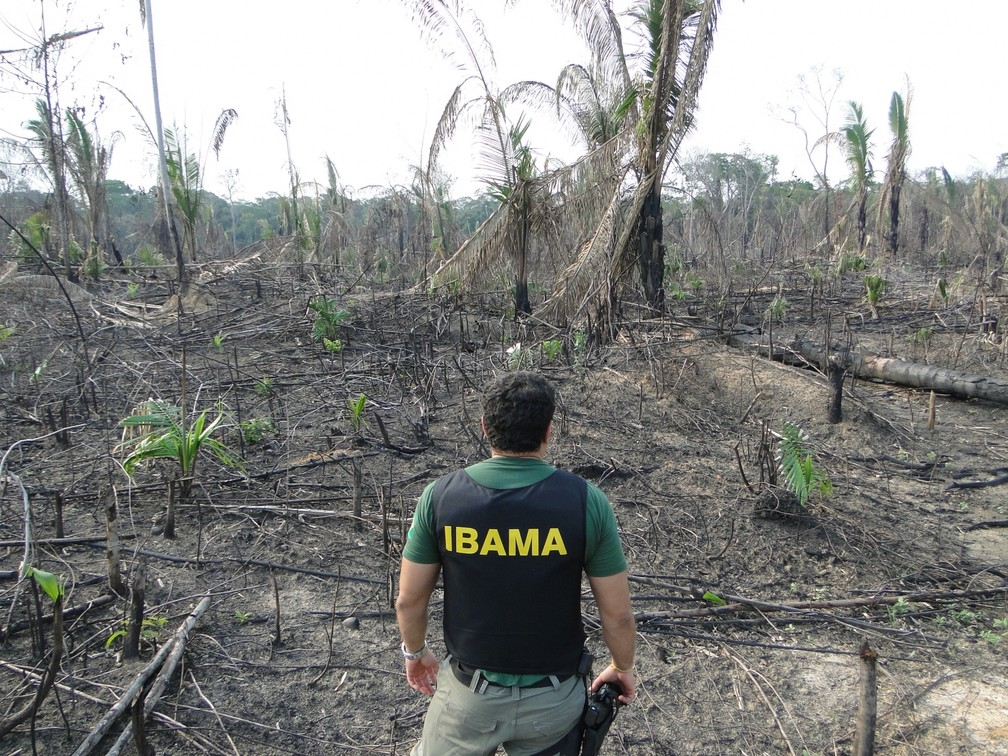
\includegraphics[width=0.9\textwidth]{img/deforestation_ibama_officer.jpg}
        \caption{Fire aftermath. Source: \href{https://g1.globo.com/natureza/noticia/2019/08/16/fim-do-lfundo-amazonia-pode-afetar-fiscalizacao-do-ibama-contra-o-desmatamento.ghtml}{Globo news}.}
        \label{fig:deforestation_ibama_officer}
      \end{figure}
    \end{column}
  \end{columns}
\end{frame}

\begin{frame}
  \frametitle{Deforestation in the Brazilian Amazon}
  \begin{columns}
    \begin{column}{0.4\textwidth}
      \begin{itemize}
        \item Current efforts are not producing the desired effect.
        \item 2021 had the highest deforestation rate since 2006 
          (~13000~\si{km^{2}}).
        % \item We need effective law enforcement actions.
      \end{itemize}
    \end{column}
    \begin{column}{0.6\textwidth}
      \begin{figure}
        \centering
        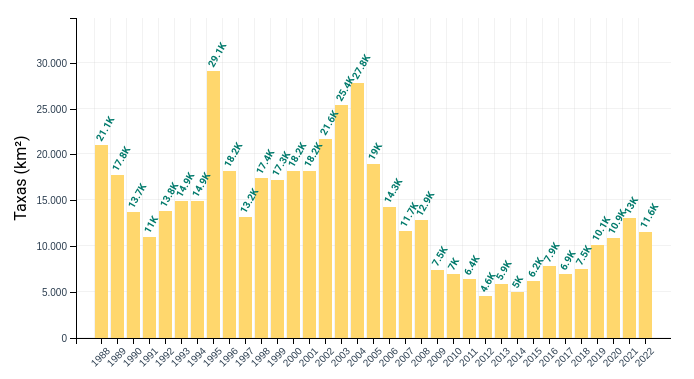
\includegraphics[width=1.0\textwidth]
        {img/prodes_deforestation_rate.png}
        \caption{Deforestation in the Brazilian Amazon (\si{\km^{2}}). Source: 
        \href{http://terrabrasilis.dpi.inpe.br/en/home-page/}{TerraBrasilis}}
        \label{fig:prodes_deforestation_rate}
      \end{figure}
    \end{column}
  \end{columns}
\end{frame}

\begin{frame}
  \frametitle{Brazil international commitments}
  \begin{columns}
    \begin{column}{0.4\textwidth}
      \begin{itemize}
        \item Reduce Greenhouse Gas emission 50\% (respect to 2005) until 2030.
        \item Zero Carbon emissions by 2050.
        \item Zero illegal deforestation by 2028.
      \end{itemize}
    \end{column}
    \begin{column}{0.6\textwidth}
      \begin{figure}
        \centering
        
\includegraphics[width=0.9\textwidth]{img/cop26_glasgow.jpg}
        % \caption{COP 26 UK 2021.}
        \label{fig:cop26}
      \end{figure}
    \end{column}
  \end{columns}
\end{frame}

\begin{frame}
  \frametitle{Brazil international commitments}
  \begin{columns}
    \begin{column}{0.4\textwidth}
      \begin{itemize}
        \item A maximum deforestation of 3925~\si{\km^{2}\per year} in 
          the Brazilian Legal Amazon, starting on 2020 (decree 9578 2018).
        \item This is similar to deforestation in 2012 (4571~\si{\km^{2}}).
      \end{itemize}
      However,
      \begin{itemize}
        \item Deforestation in 2021 was 271\% of this commitment.
      \end{itemize}
    \end{column}
    \begin{column}{0.6\textwidth}
      \begin{figure}
        \centering
        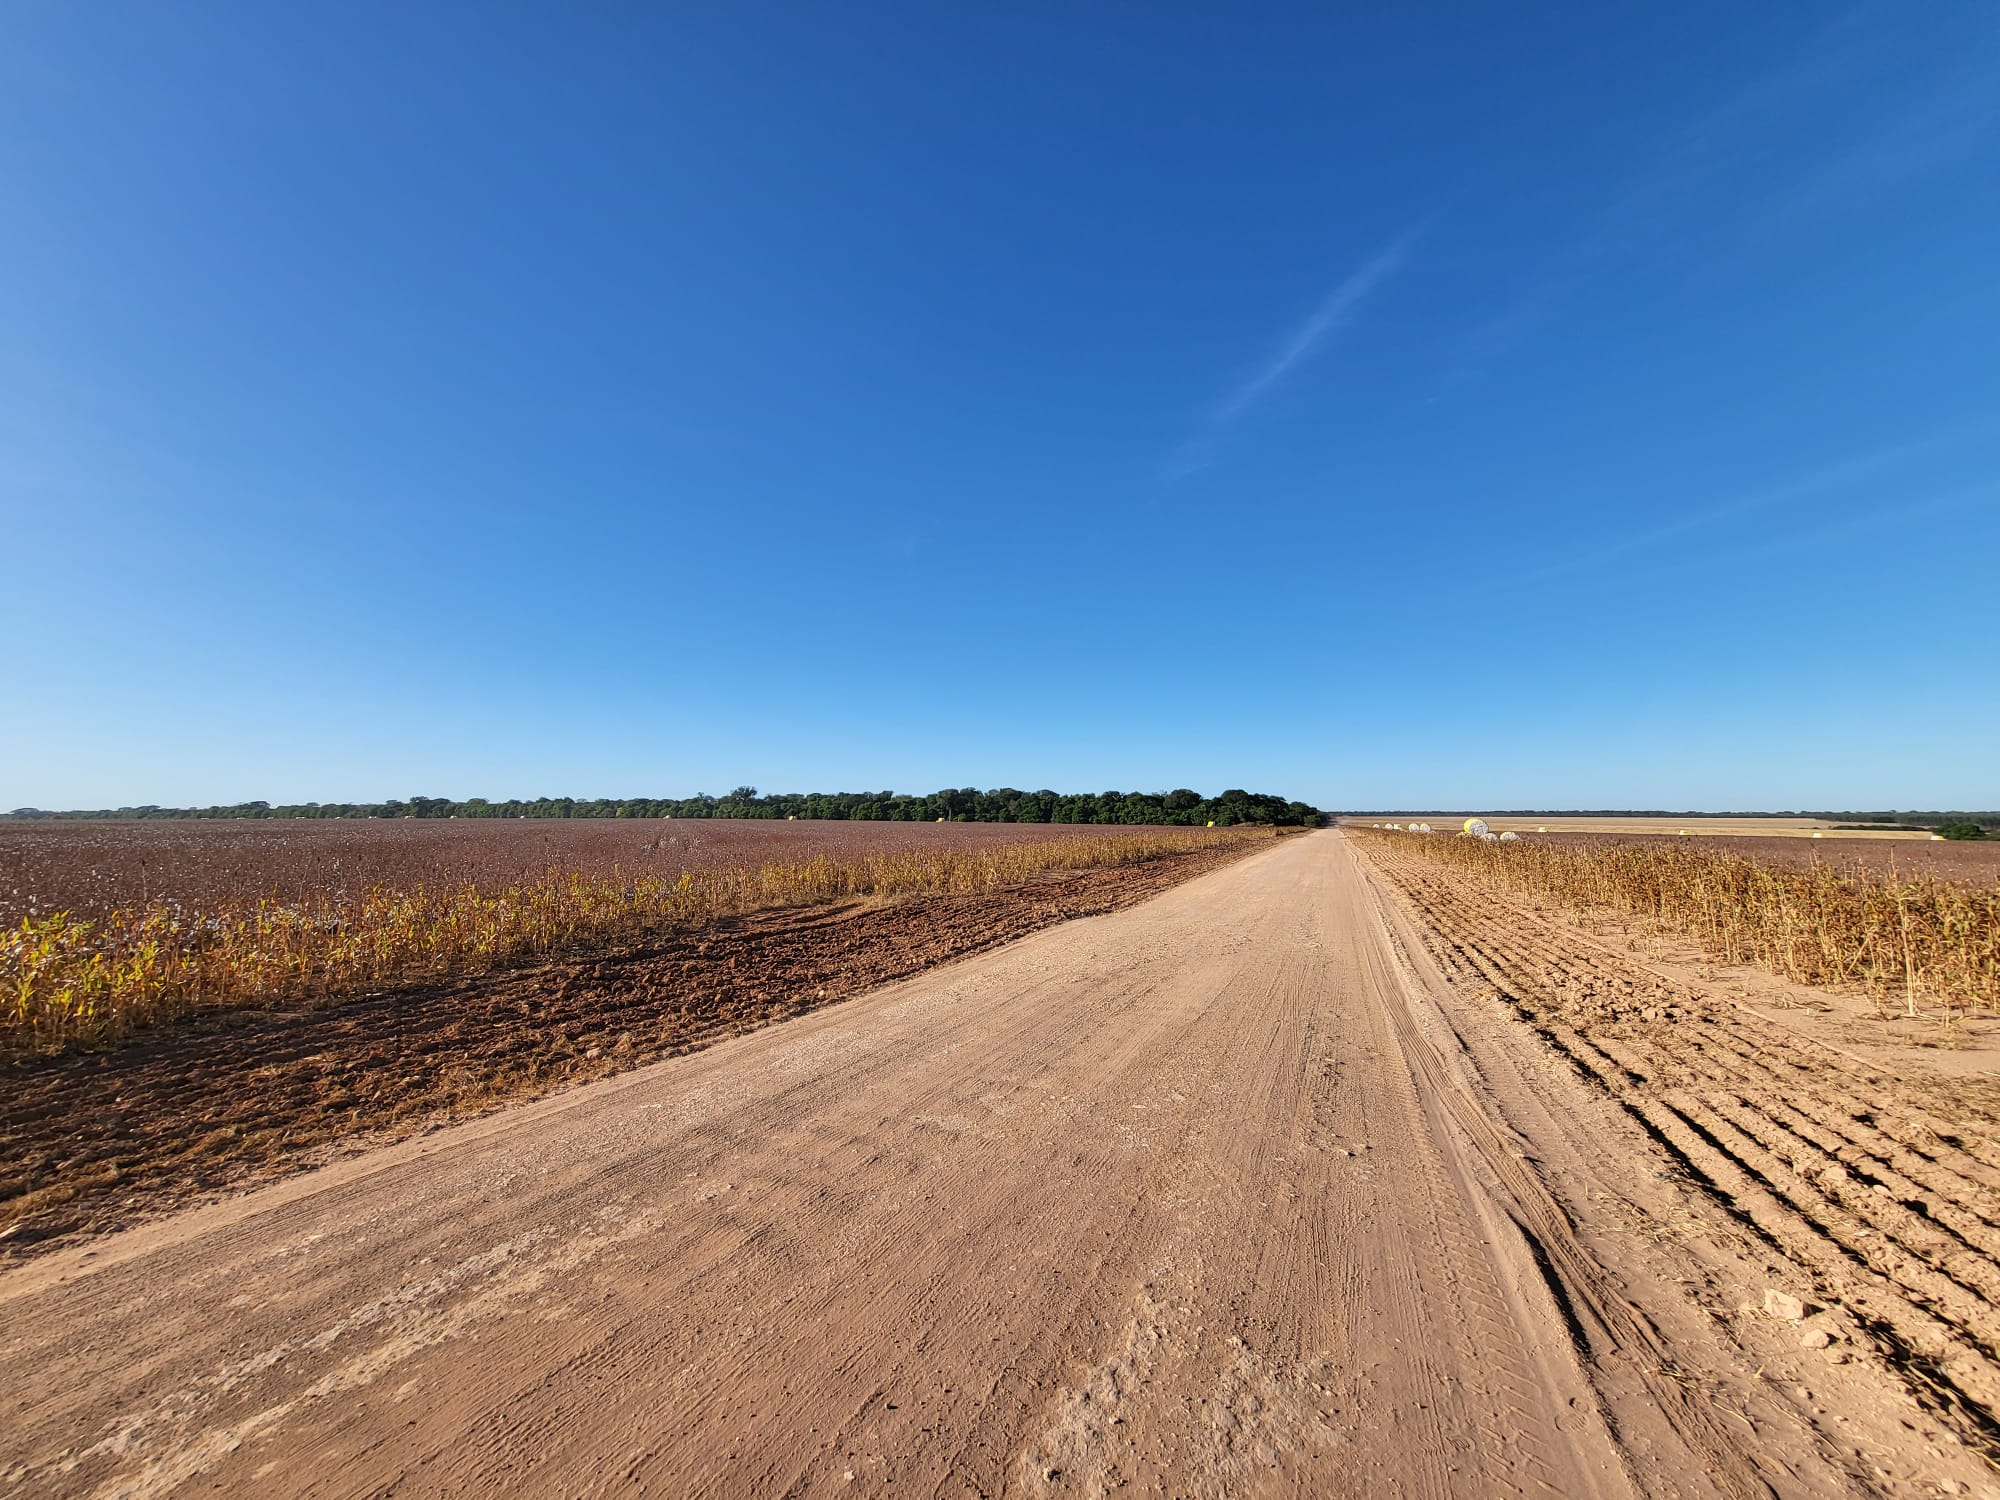
\includegraphics[width=0.9\textwidth]{img/planted_field.png}
        %\caption{Planted field (cotton). Source: INPE}
        \caption{Source: INPE}
        \label{fig:planted_field}
      \end{figure}
    \end{column}
  \end{columns}
\end{frame}


\section{Fire}

% TODO: How to smootly transition from deforestaion to fire?

\begin{frame}
  \frametitle{Fire in the Amazon}
  \begin{figure}
    \centering
    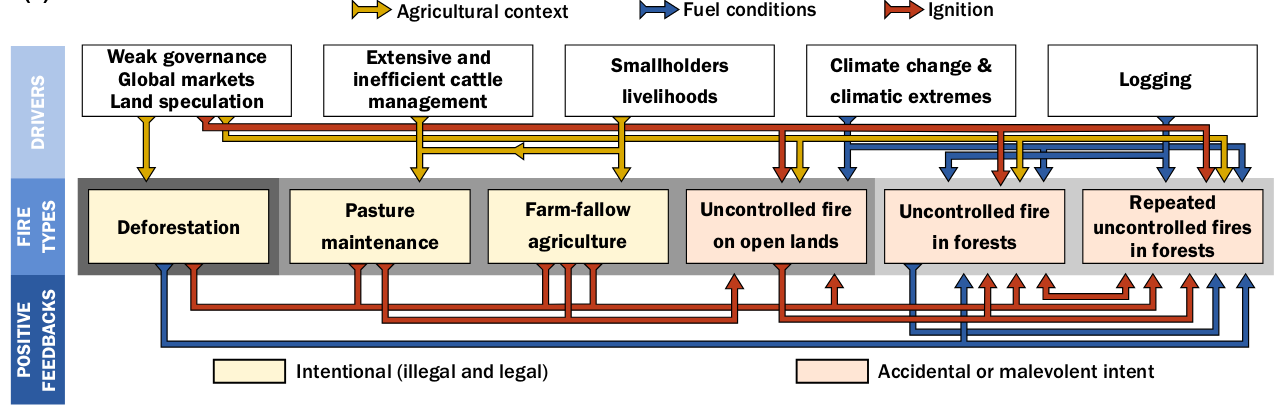
\includegraphics[width=0.9\textwidth]
    {img/amazonian_fires_drivers_types_feedbacks.png}
    \caption{Overview of fire drivers, types and feedbacks. 
             Source:~\cite{barlow2020}}
    \label{fir:fire_drivers}
  \end{figure}
\end{frame}

\begin{frame}
  \frametitle{Types of fire}
  \begin{columns}
    \begin{column}{0.4\textwidth}
      \begin{itemize}
        \item Deforestation fire.
        \item Understory forest fire.
        \item Clearing \& Agricultural fire.
        \item Savanna fire.
      \end{itemize}
    \end{column}
    \begin{column}{0.6\textwidth}
      \begin{figure}
        \centering
        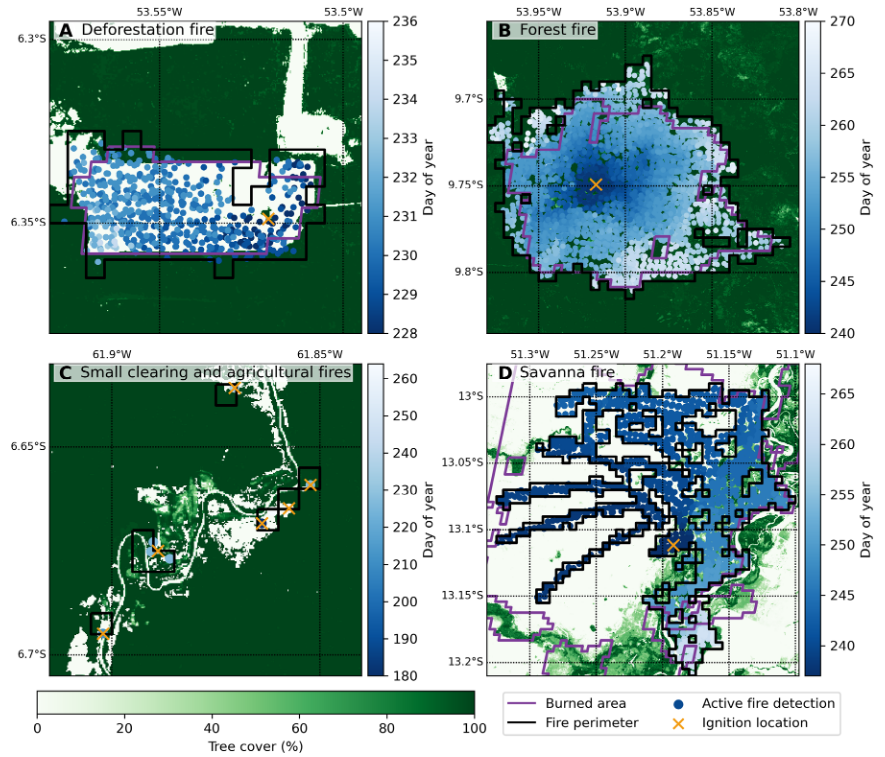
\includegraphics[width=0.95\textwidth]{img/fire_types.png}
        \caption{Dominant fire types in the Amazon. Source~\cite{andela2022}.}
      \end{figure}
    \end{column}
  \end{columns}
\end{frame}

\begin{frame}
  \frametitle{Biomass burning}
  \begin{columns}
    \begin{column}{0.4\textwidth}
      \begin{itemize}
        \item plays a role in the biosphere-atmosphere interaction.
        \item harms the human health.
        \item leads to economic losses.
        \item contributes to climate change~\cite{thornhill2018}.
      \end{itemize}
    \end{column}
    \begin{column}{0.6\textwidth}
      \begin{figure}
        \centering
        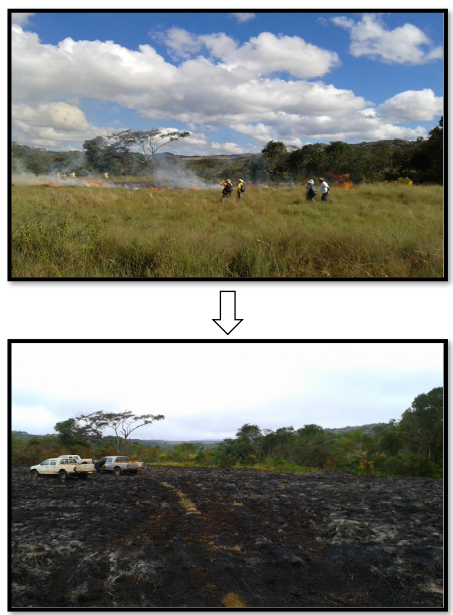
\includegraphics[width=0.5\textwidth]{img/grass_on_fire.png}
        \caption{Source: INPE}
        \label{fig:grass_on_fire}
      \end{figure}
    \end{column}
  \end{columns}
\end{frame}

% \begin{frame}
%   \frametitle{Biomass burning (BB) emissions}
%   \begin{columns}
%     \begin{column}{0.4\textwidth}
%       \begin{itemize}
%         \item 2.2\si{\peta\gram} of Carbon are emitted annually by BB
%           (1\si{\peta\gram} are $10^{12}$\si{\kilogram}).
%         \item Most Carbon emissions in savannas are associated to BB 
%           (GFED 4.1s)~\cite{randerson2017a}.
%         \item BB emissions by deforestation in the tropics account for 15\% of 
%           annual emissions and are increasing (GFED 4.1s).
%         \item 15\% of the Carbon emitted from 1997 to 2019 occurred
%           in South America (GFED 4.1s).
%       \end{itemize}
%     \end{column}
%     \begin{column}{0.6\textwidth}
%       \begin{figure}
%         \centering
%         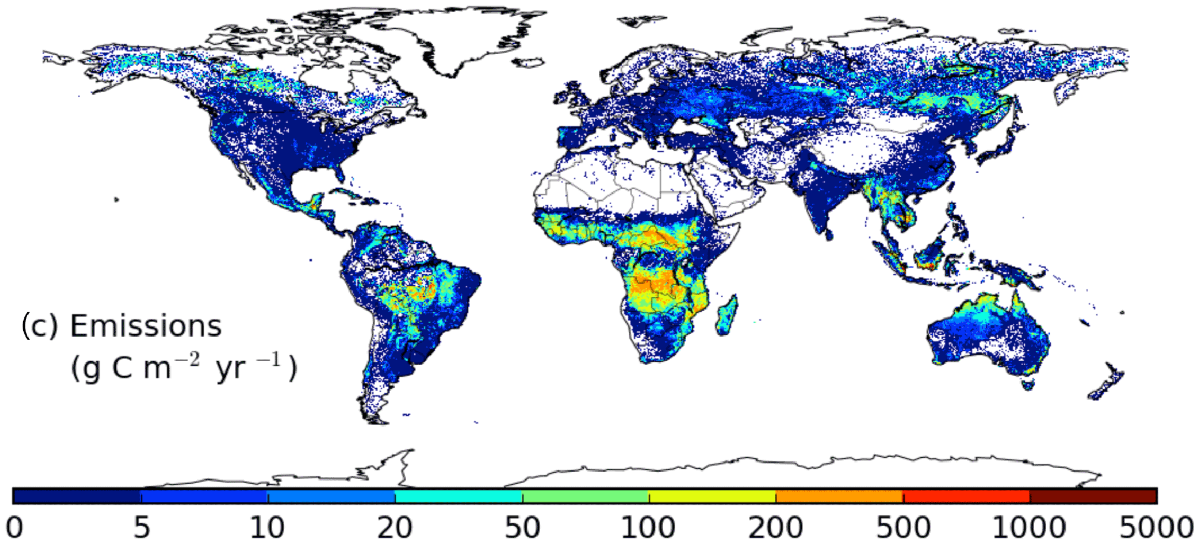
\includegraphics[width=0.9\textwidth]{img/gfed4s_emissions.png}
%         \caption{GFED4s emissions averages over 1997-2016. 
%         Source~\cite{vanderwerf2017}.}
%         \label{fig:gfed4s_emissions}
%       \end{figure}
%     \end{column}
%   \end{columns}
% \end{frame}

\begin{frame}
  \frametitle{Biomass burning emissions in Brazil}
  \begin{columns}
    \begin{column}{0.4\textwidth}
      \begin{itemize}
        \item BB emissions by deforestation in the tropics account for 15\% of 
          annual emissions and are increasing (GFED 4.1s).
        \item 15\% of the Carbon emitted from 1997 to 2019 occurred
          in South America (GFED 4.1s).
        \item 60\% of the South American BB emissions occur in the Brazilian
          territory~\cite{santos2021}.
        \item Concentrated in the Amazon and Cerrado biomes.
        \item Mostly driven by land use and land cover change.
      \end{itemize}
    \end{column}
    \begin{column}{0.6\textwidth}
      \begin{figure}
        \centering
        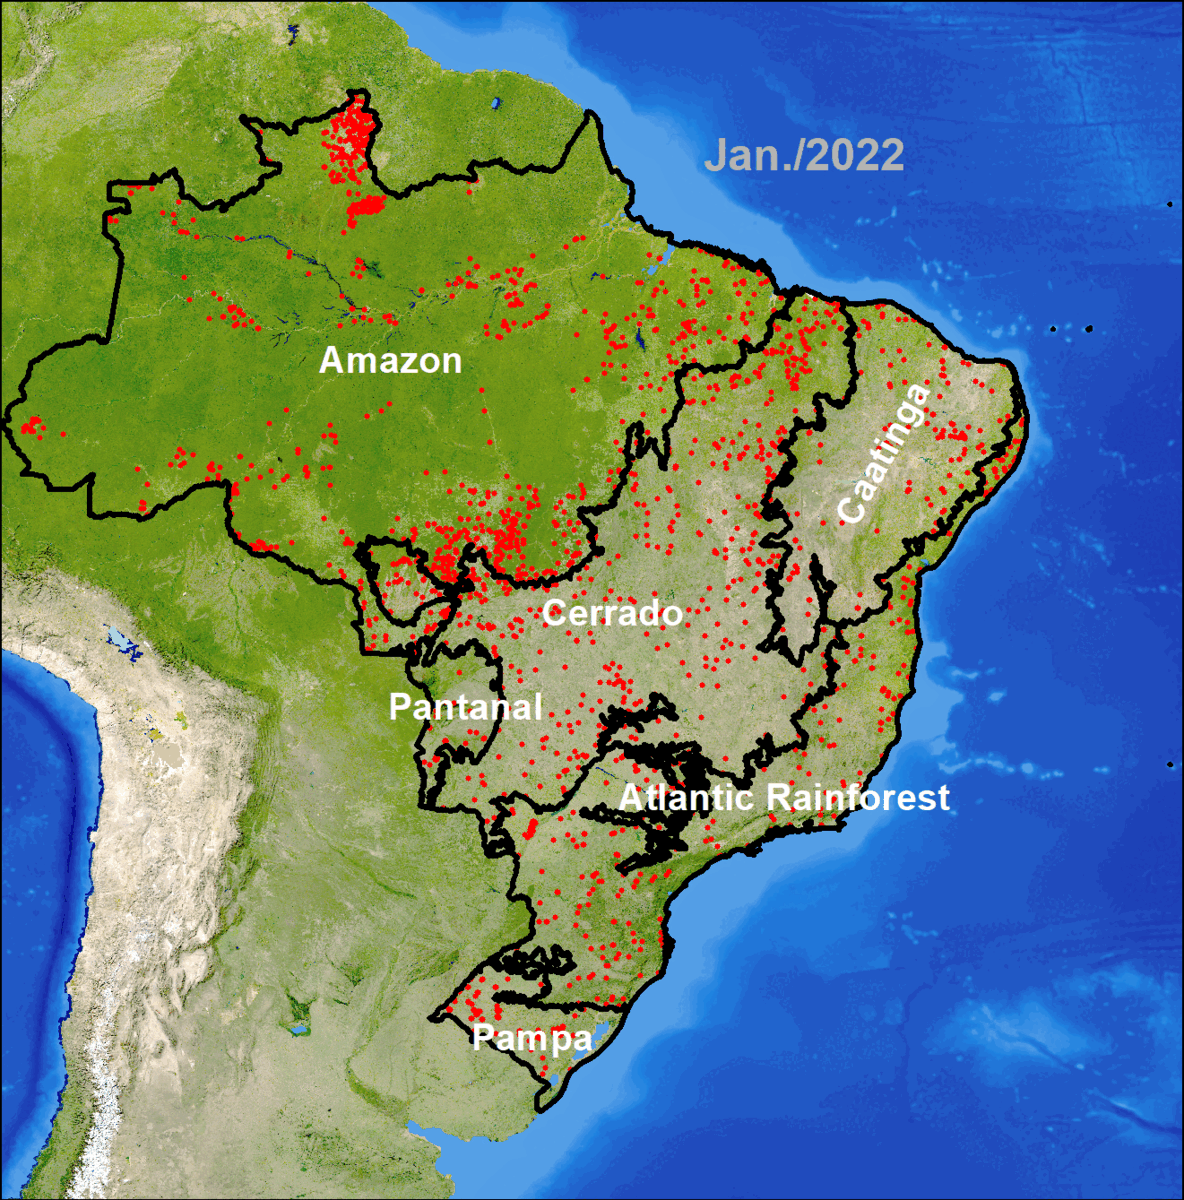
\includegraphics[width=0.6\textwidth]{img/monthly_active_fires.png}
        \caption{Monthly active fires detected by MODIS-Aqua in January 2022. 
        Source: INPE}
        \label{fig:monthly_active_fires}
      \end{figure}
    \end{column}
  \end{columns}
\end{frame}

\begin{frame}
  \frametitle{Fire spots by month (VIIRS satellite)}
    \begin{figure}[h] 
        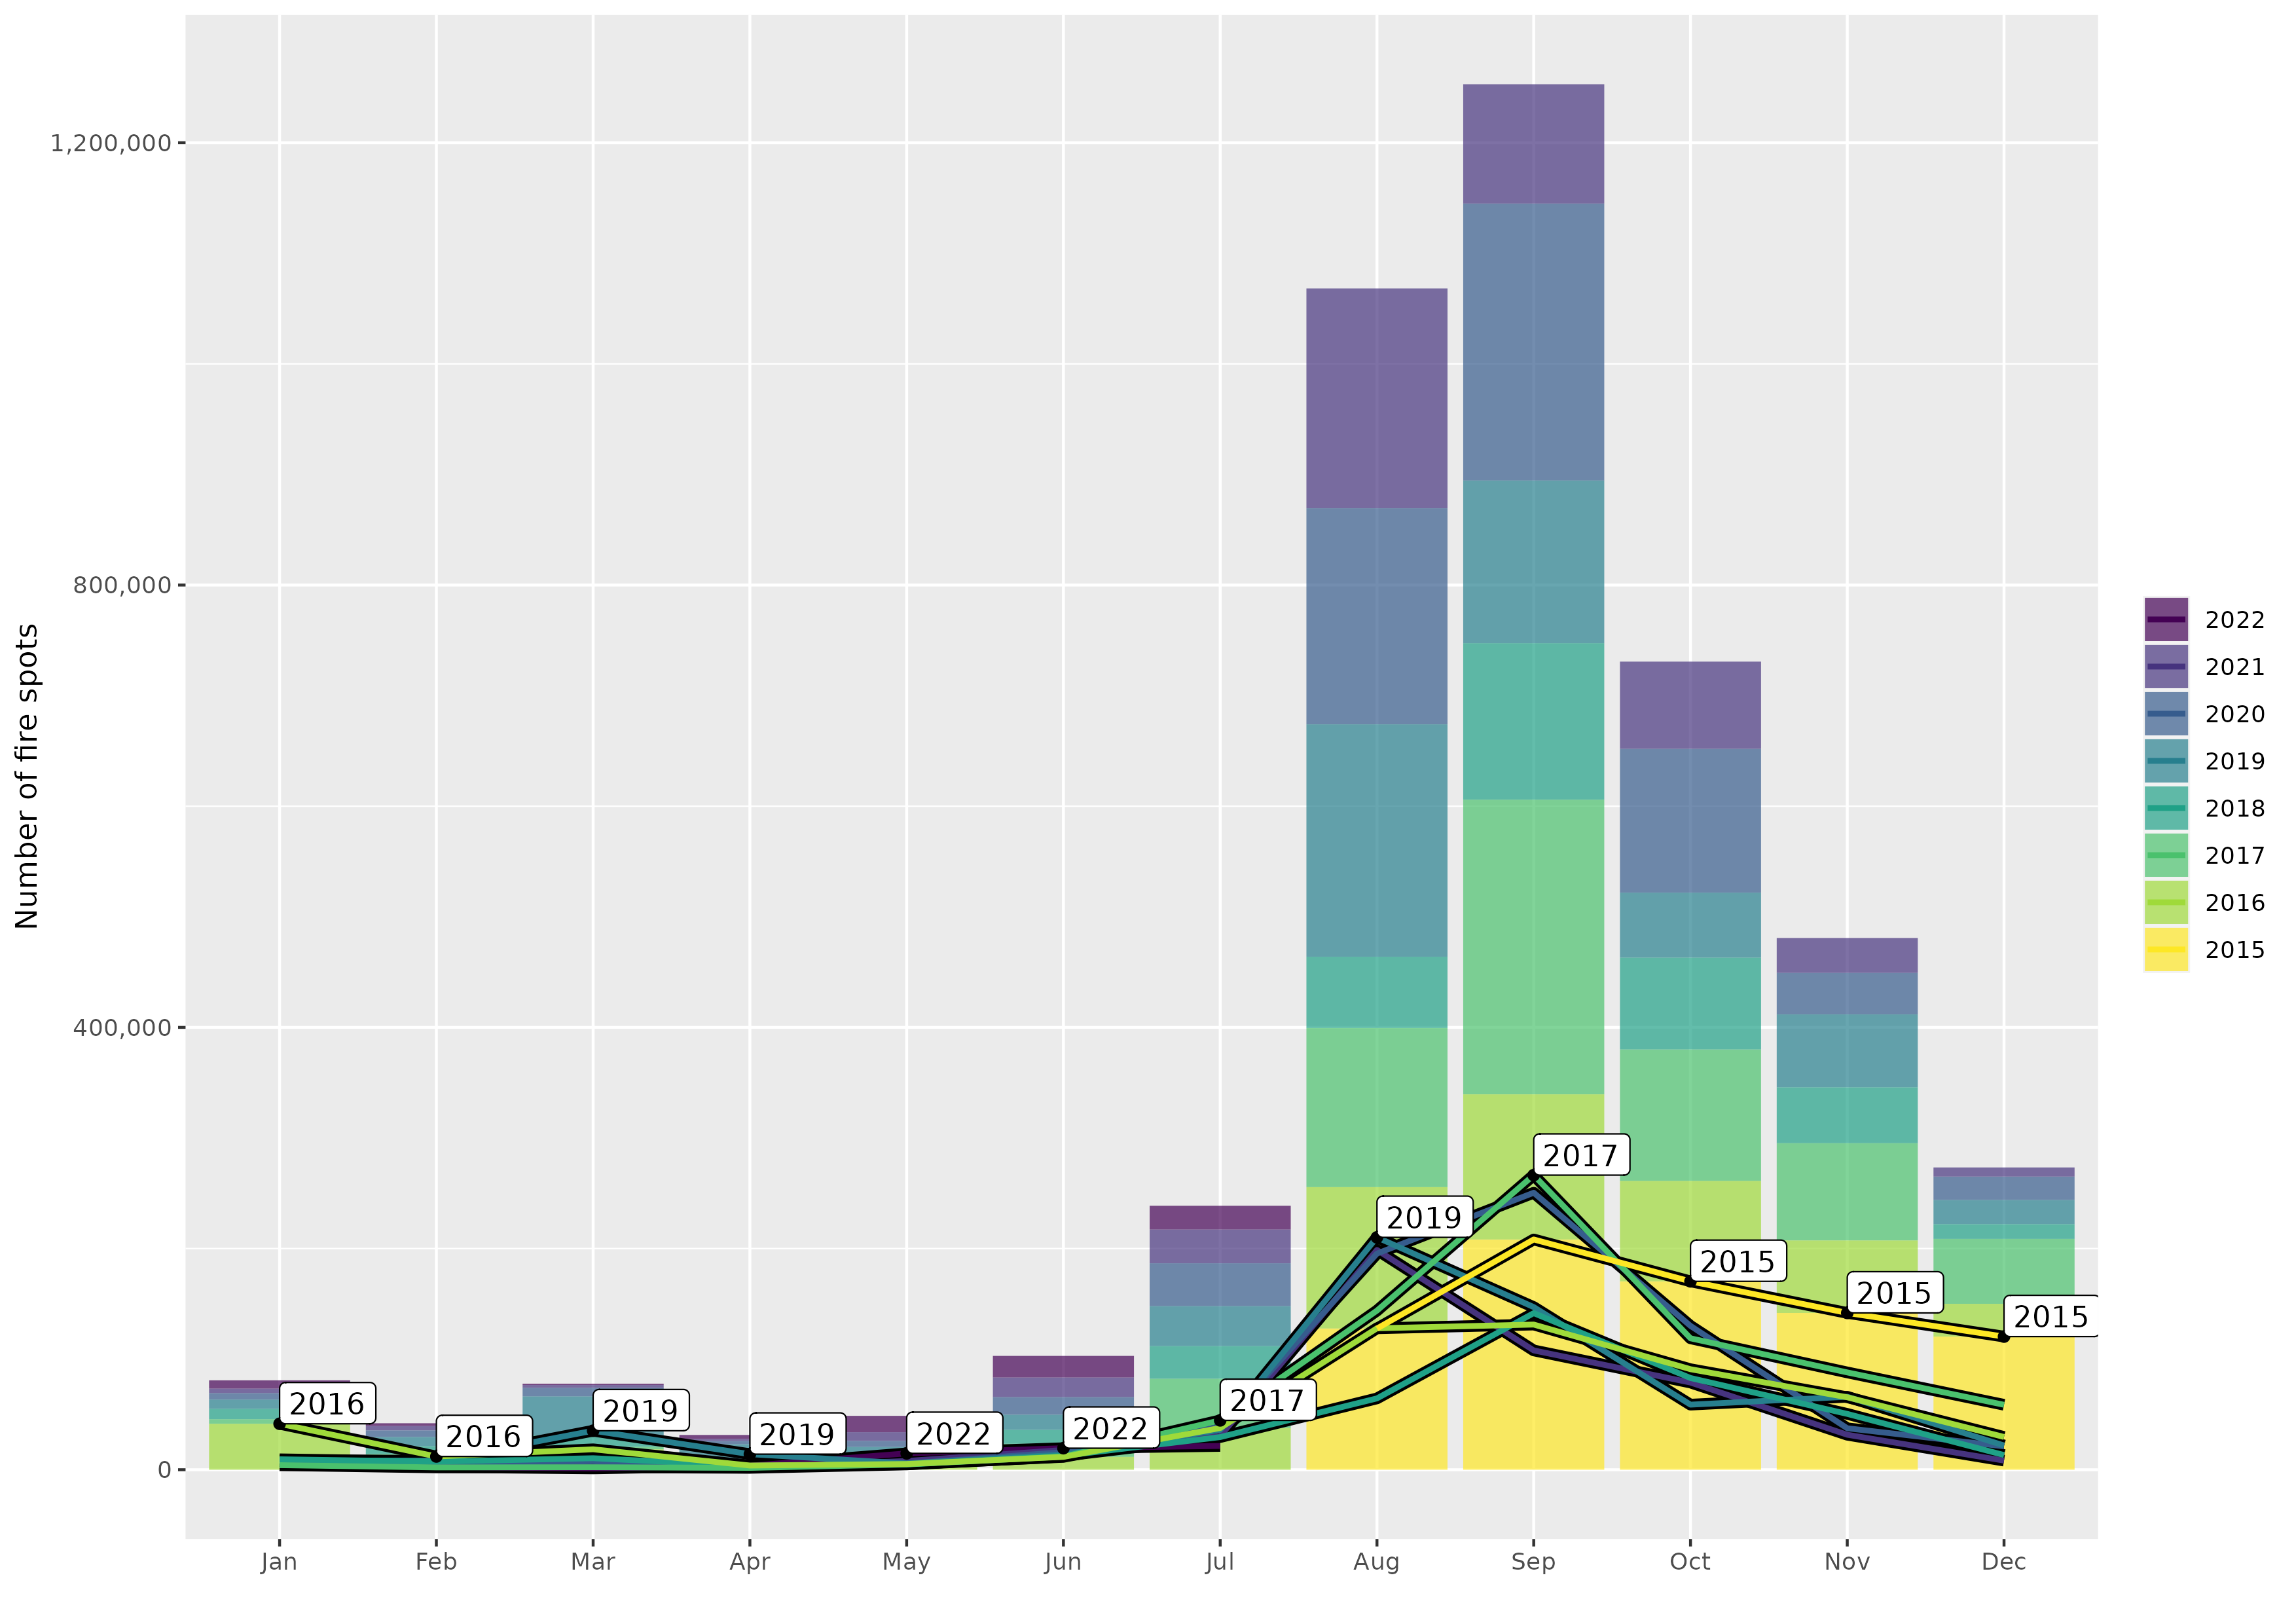
\includegraphics[width=0.65\textwidth] 
        {./figures/plot_fire_spots_by_month.png} 
        \caption{Aug (2019) \& Sep (2017) top fire spots. 
        Note 2015's last trimester.}
    \end{figure}
\end{frame}

\begin{frame}
    \frametitle{Fire spots by month and state}
    \begin{figure}[h]
        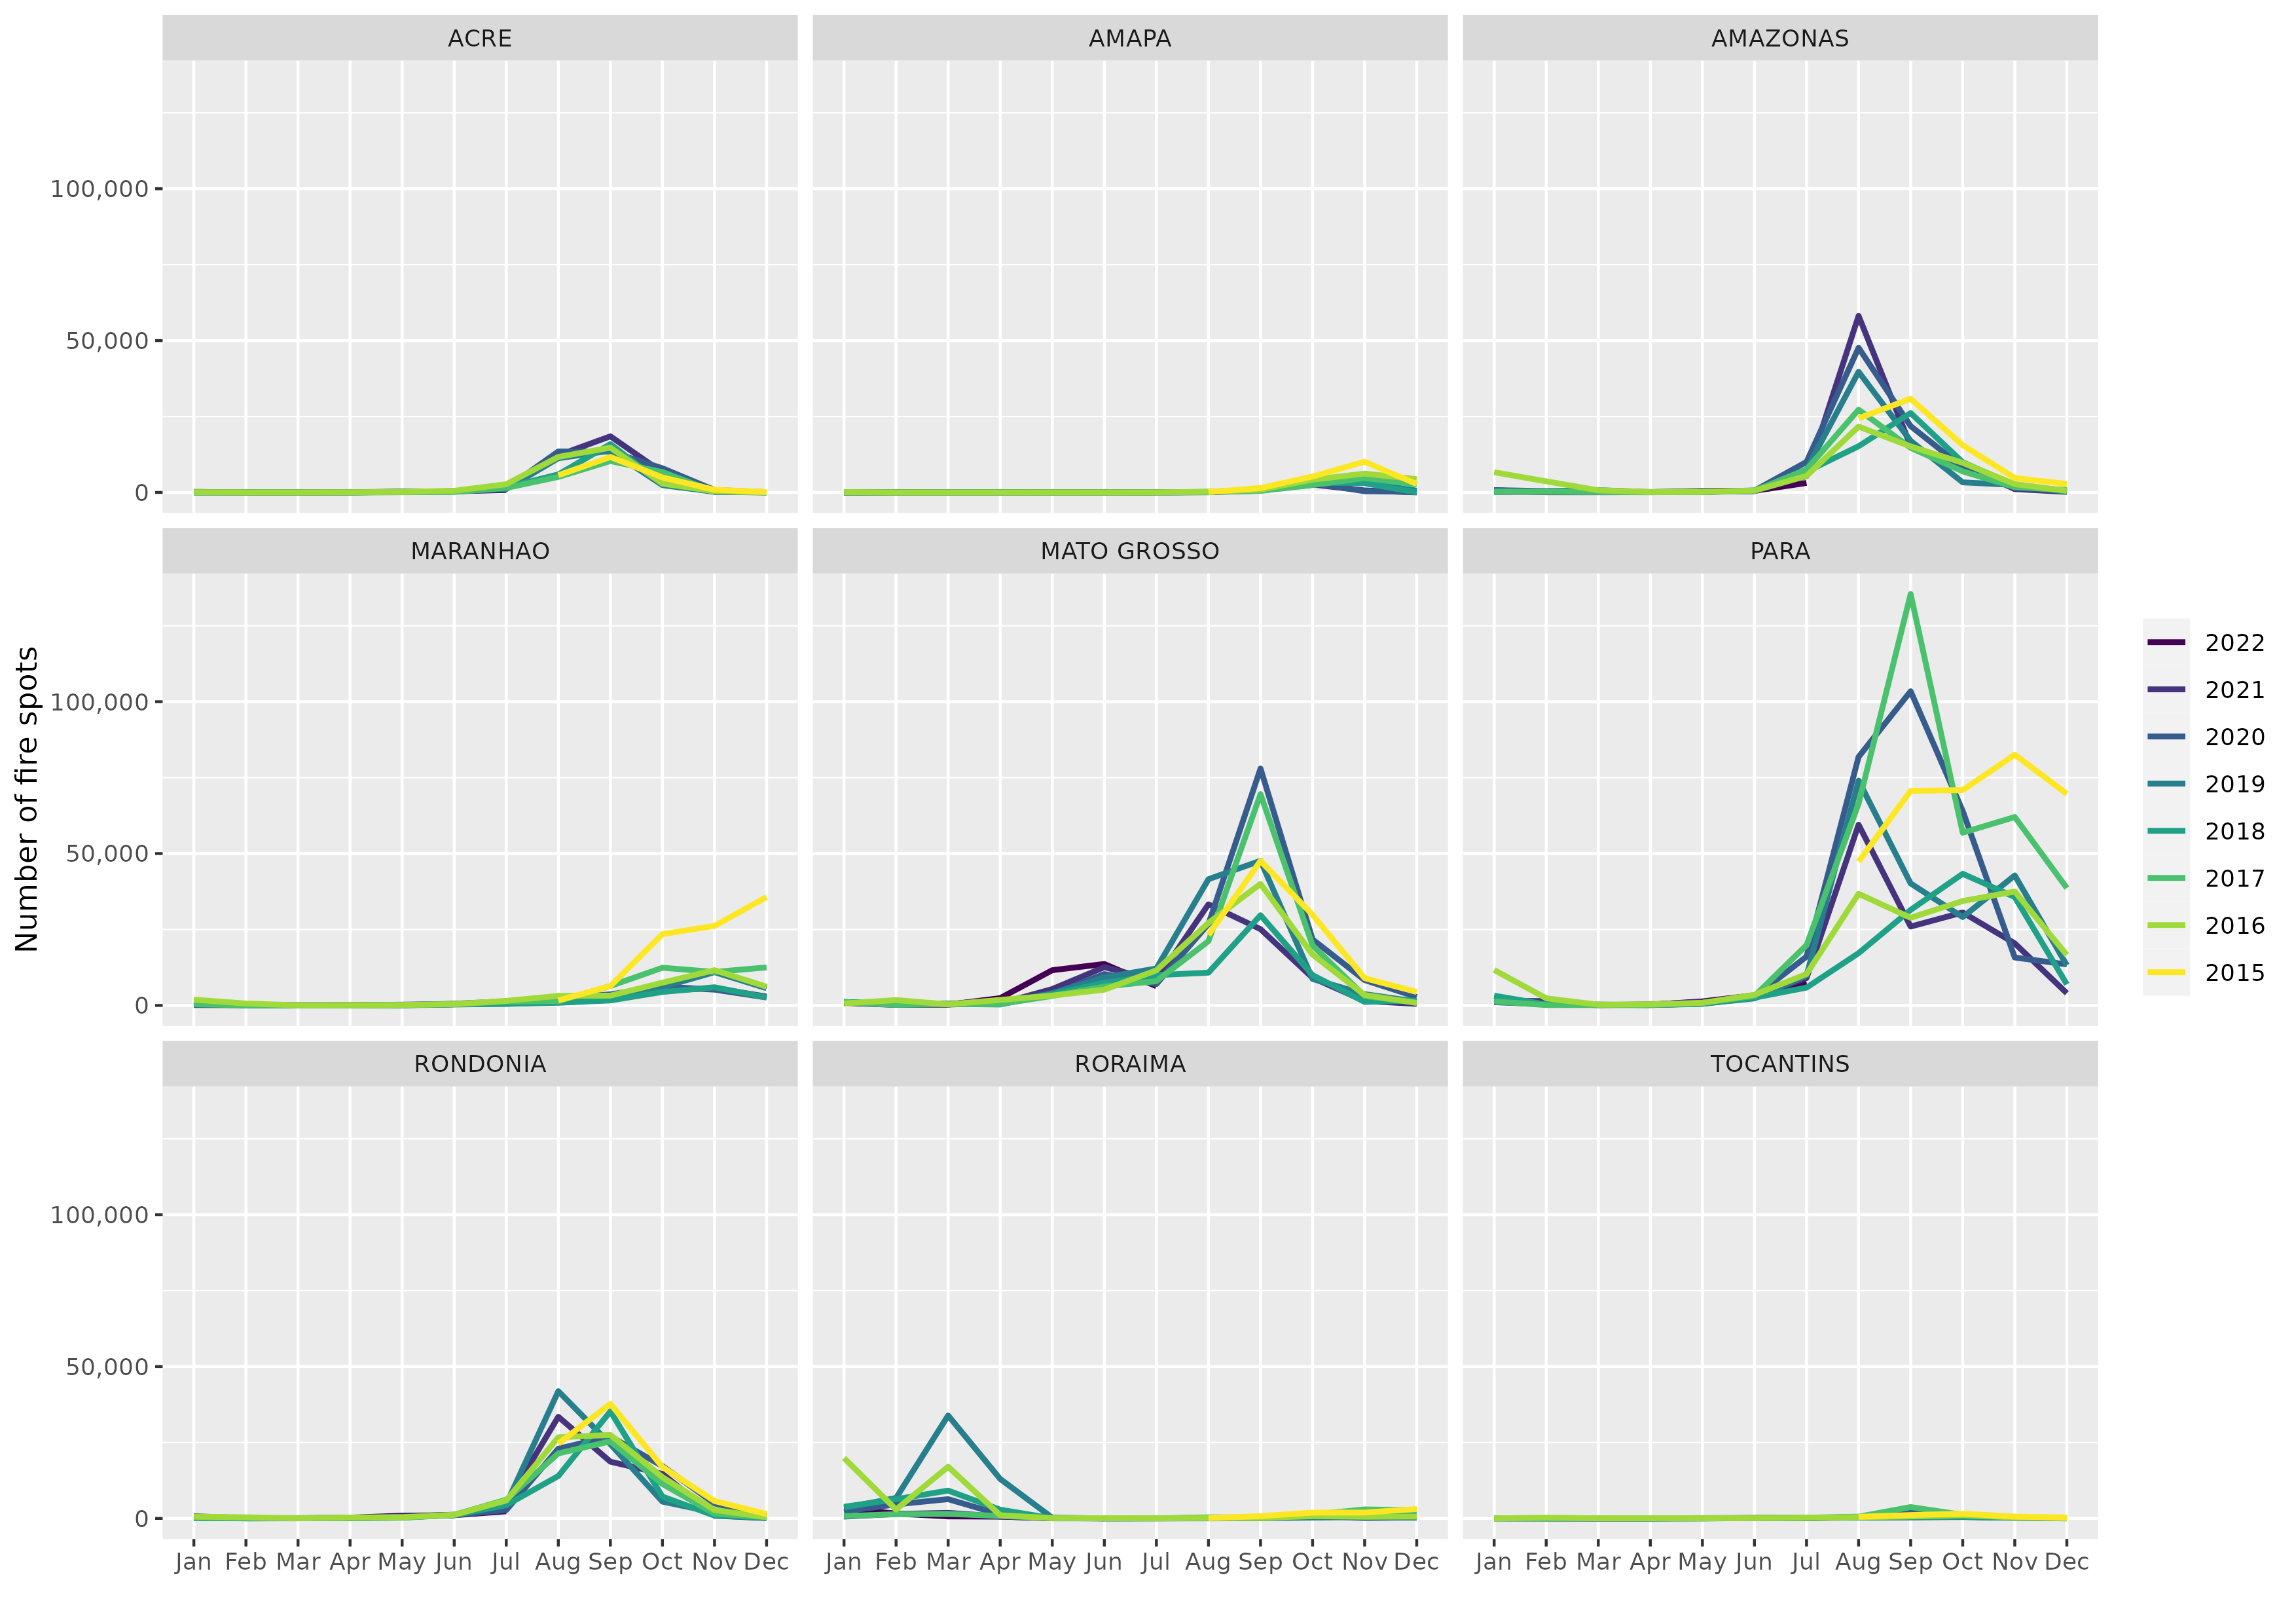
\includegraphics[width=0.65\textwidth]
        {./figures/plot_fire_spots_by_month_state.png}
        \caption{Note the incresing trend in Amazonas and its move towards
        August.}
    \end{figure}
\end{frame}

% \begin{frame}
%     \frametitle{Fire spots density (by area overlap with BLA)}
%     \begin{figure}[h]
%         \includegraphics[width=0.65\textwidth]
%         {./figures/plot_fire_spots_density_by_state.png}
%         \caption{Number of fire spots by state and their density (by 
%         area in BLA).}
%     \end{figure}
% \end{frame}


\section{DETER}


\begin{frame}
  \frametitle{INPE's information systems}
  \begin{columns}
    \begin{column}{0.4\textwidth}
      \begin{itemize}
        \item PRODES: Deforestation accounting.
        \item DETER: Issue deforestation warnings.
        \item TerraClass: Deforestation follow-up.
      \end{itemize}
    \end{column}
    \begin{column}{0.6\textwidth}
      \begin{figure}
        \centering
        
\includegraphics[width=0.7\textwidth]{logos/Inpelogo.png}
      \end{figure}
    \end{column}
  \end{columns}
\end{frame}

\begin{frame}
    \frametitle{DETER}
    \begin{columns}
      \begin{column}{0.4\textwidth}
        \begin{itemize}
            \item DETER is a GIS which produces a fast assessment of 
              deforestation and forest degradation in the Brazilian 
              Amazon~\cite{Shimabukuro:2006}.
            \item DETER employs Linear Mixture Models of CBERS imagery and 
              human experts to deter and issue warnings of deforested 
              (or degraded) areas larger than 3 ha~\cite{dealmeida2022}.
            % \item Annually, DETER takes from PRODES the current forested area, 
            %   stating anew issuing warnings.
        \end{itemize}
      \end{column}
      \begin{column}{0.6\textwidth}
        \begin{figure}
          \centering
          
\includegraphics[width=1.2\textwidth]{logos/deterblogo.jpg}
        \end{figure}
      \end{column}
    \end{columns}
\end{frame}

\begin{frame}
    \frametitle{DETER warnings}
    \begin{figure}[h] 
        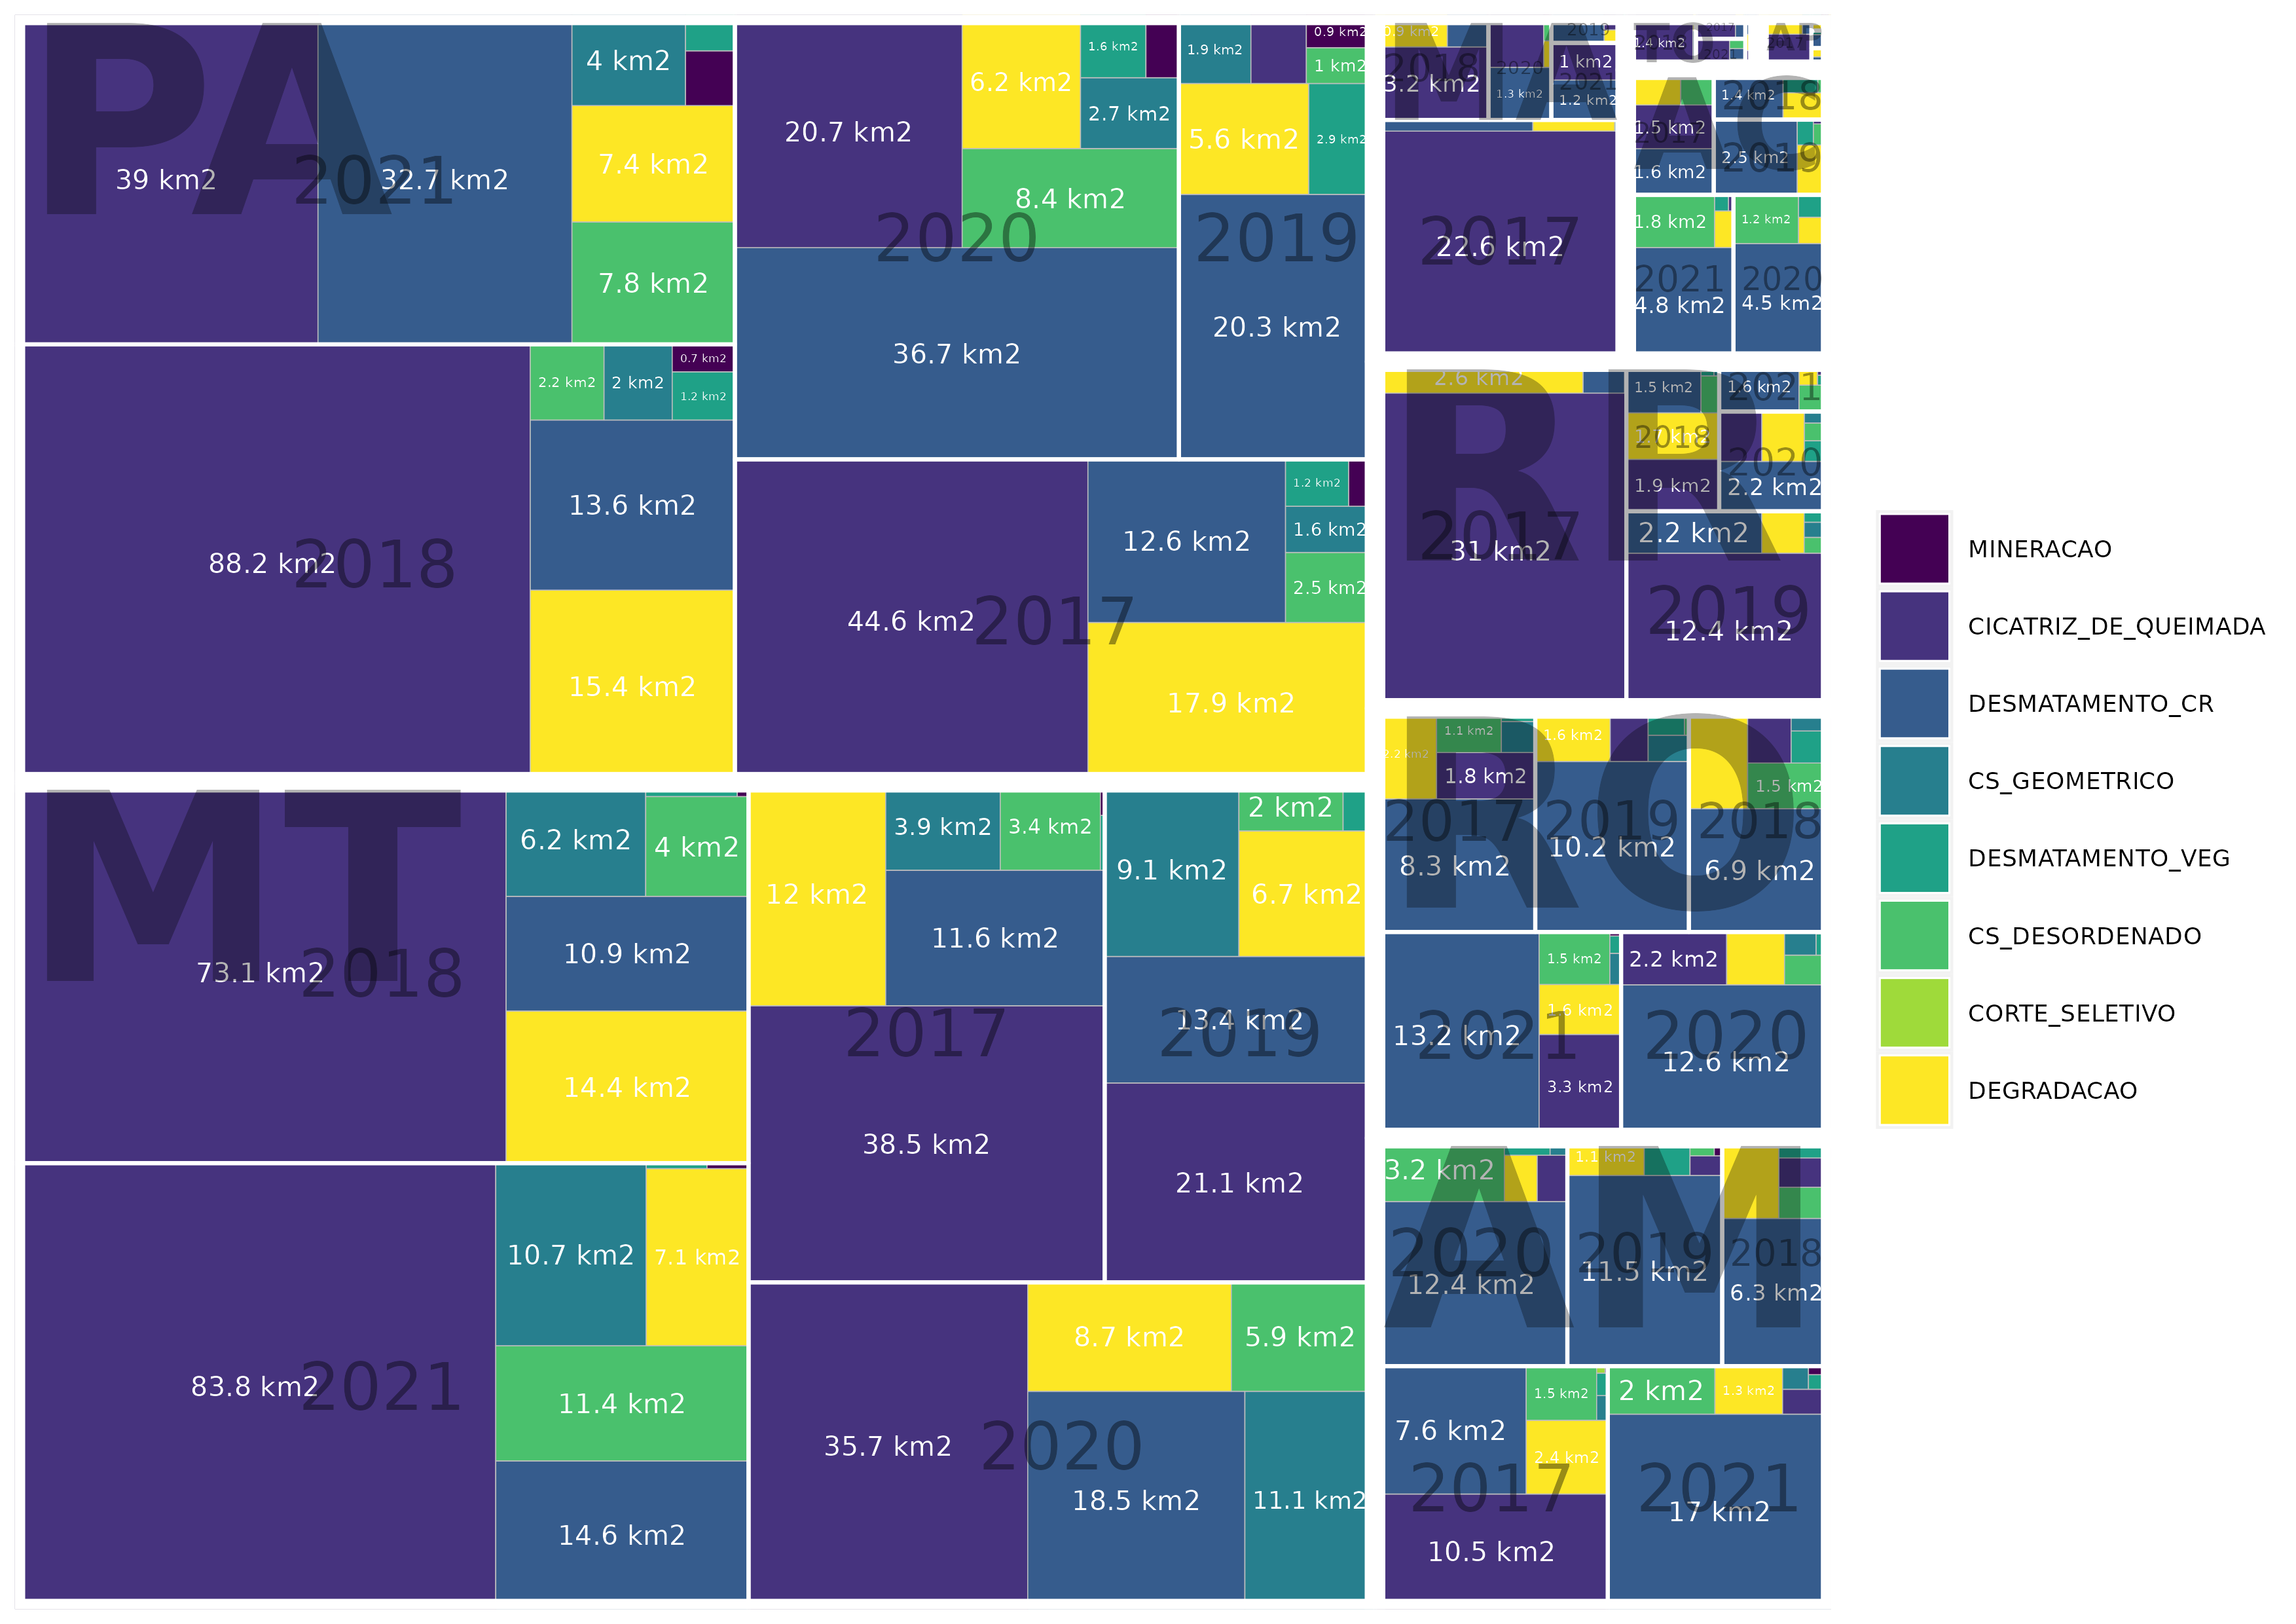
\includegraphics[width=0.75\linewidth]
        {figures/plot_deter_area_by_state_pyear_type.png}
        \label{fig:deter_area_state_pyear_type}
    \end{figure}
\end{frame}

\begin{frame}
    \frametitle{DETER warnings by class}
    \begin{figure}[h]
        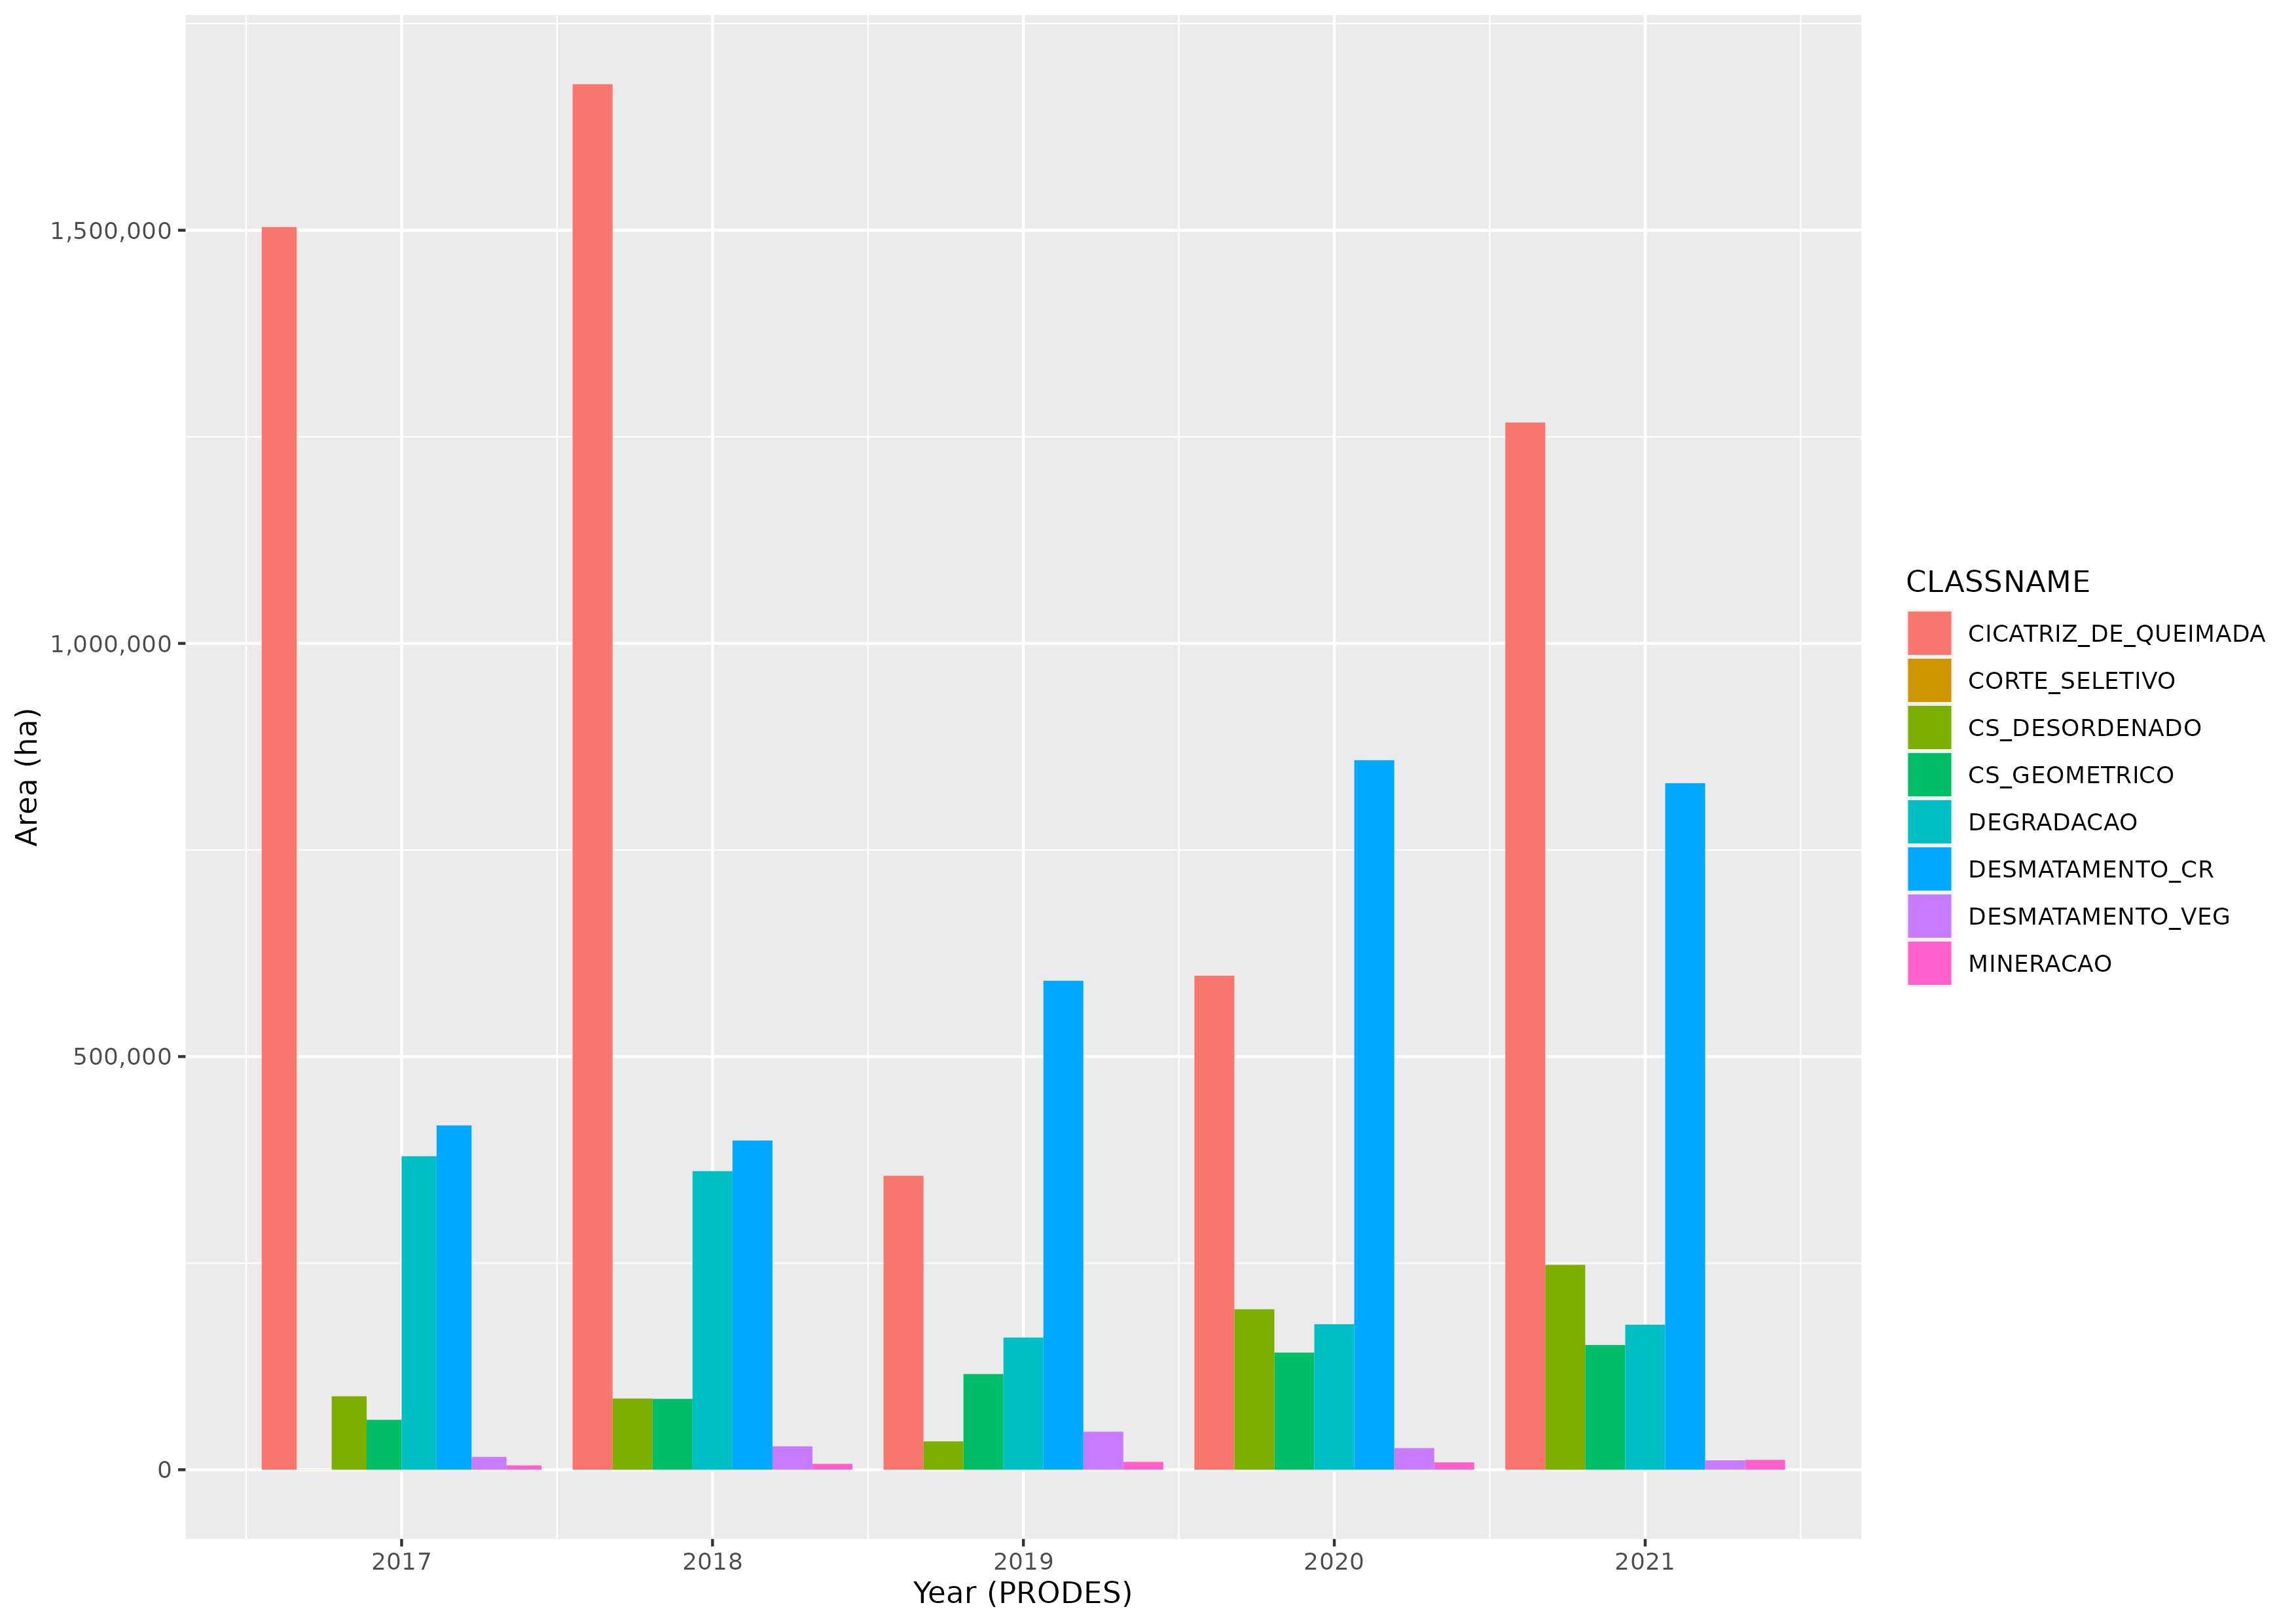
\includegraphics[width=0.65\linewidth]
        {figures/plot_deter_area_by_class.png}
        \label{fig:deter_area_by_class}
        \caption{Burn scars and clear cut are the most common warnings.}
    \end{figure}
\end{frame}

\begin{frame}
    \frametitle{DETER warnings by class and state}
    \begin{figure}[h]
        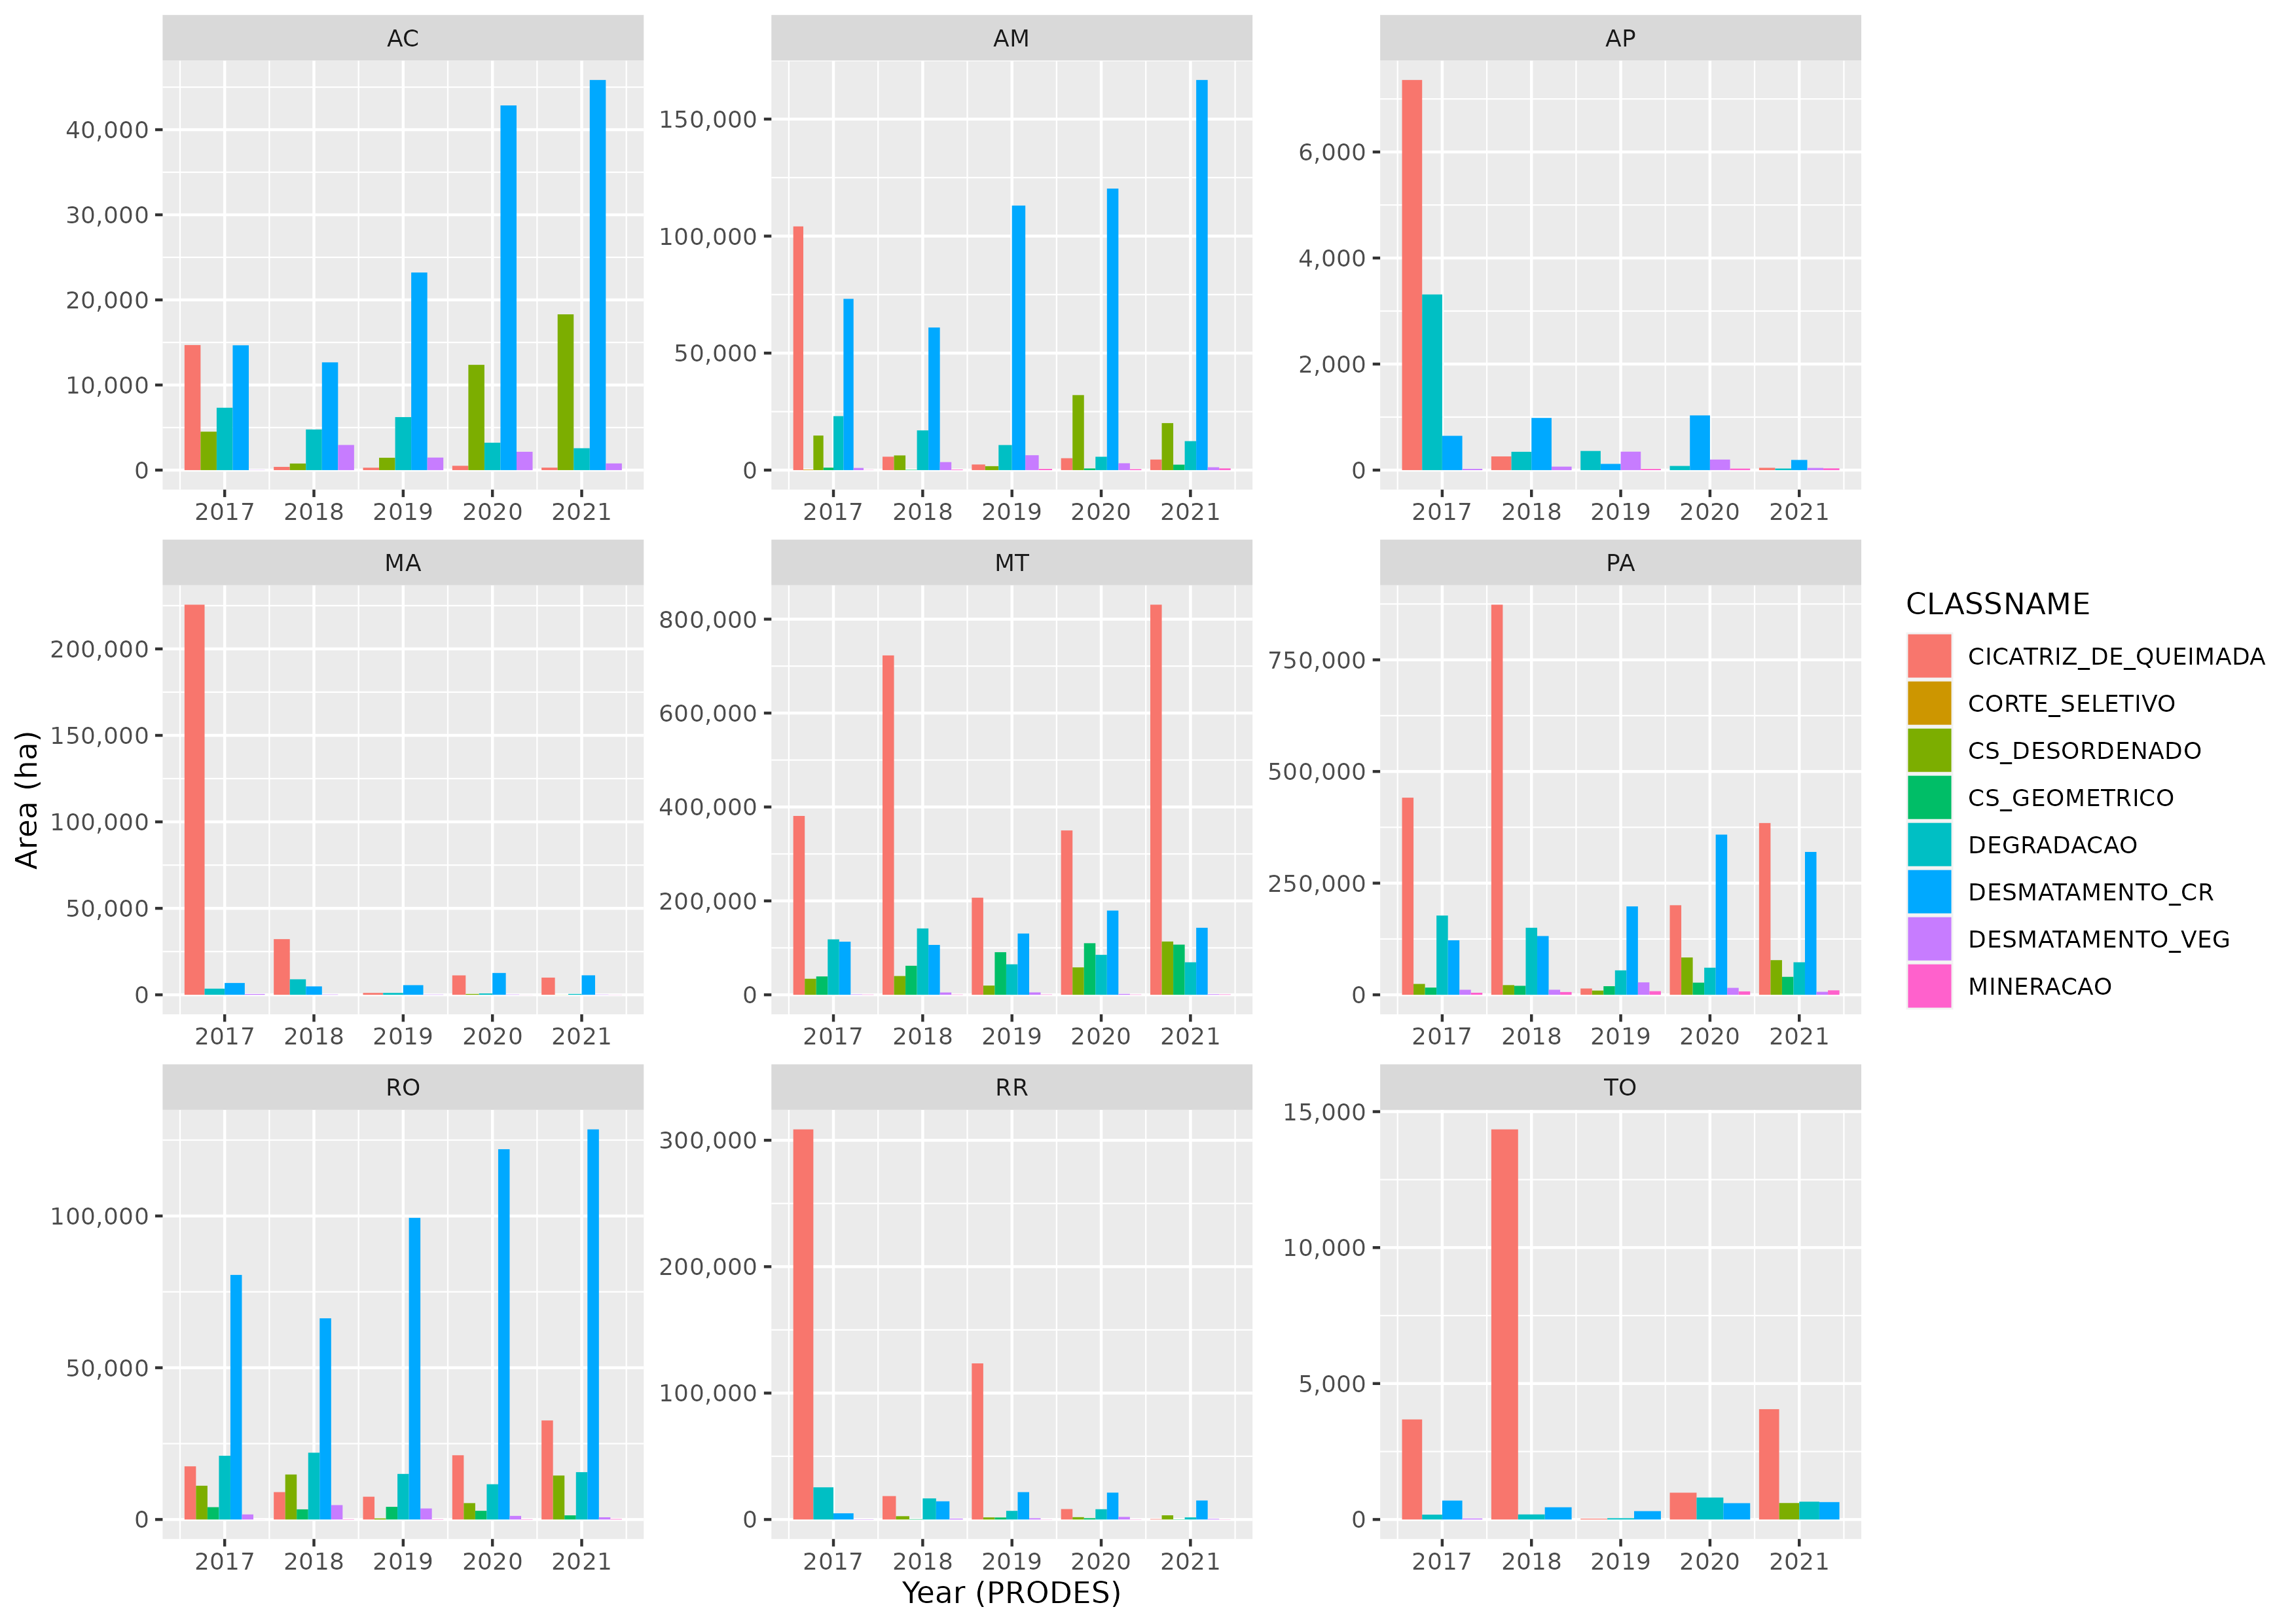
\includegraphics[width=0.65\linewidth]
        {./figures/plot_deter_area_by_class_state.png}
        \label{fig:deter_area_by_class_state}
        \caption{Burn scars and clear cut are the most common warnings.}
    \end{figure}
\end{frame}

\begin{frame}
    \frametitle{DETER warnings and time}
    \begin{itemize}
        \item The spatial properties of DETER warning are inconsistent along 
            time (shape, size, position, orientation).
    \end{itemize}
\end{frame}

\begin{frame}
    \frametitle{Warnings are inconsistent along time}
    \begin{figure}[h] 
        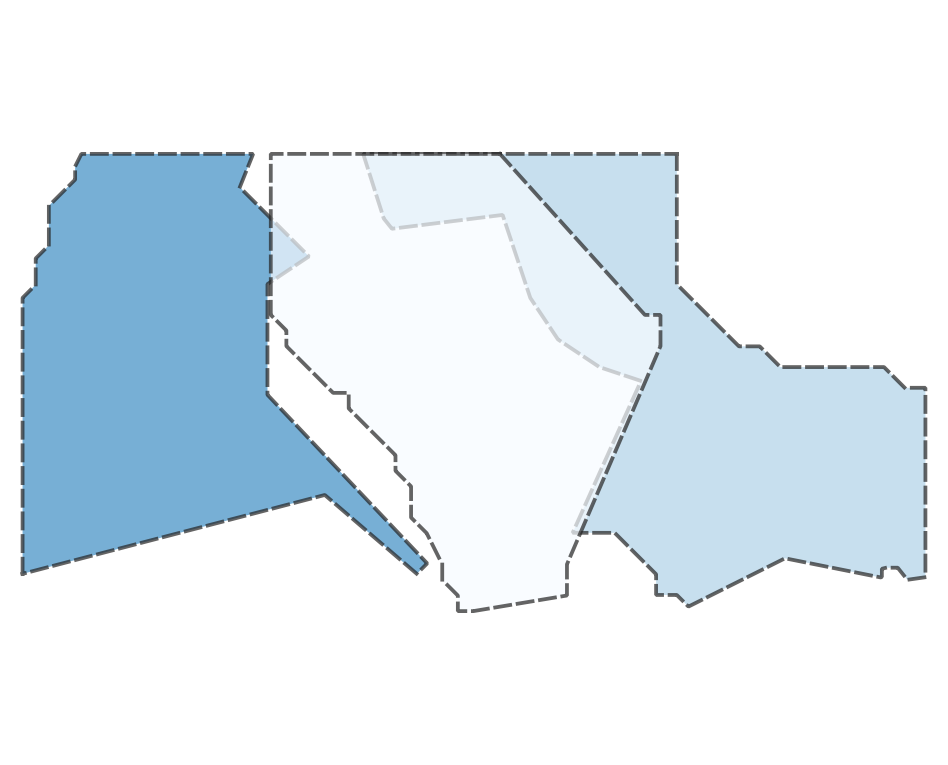
\includegraphics[width=0.60\linewidth]
        {img/sample_deter_warnings.png}
        \label{fig:deter_subareas}
        \caption{DETER warnings don't fit along time.}
    \end{figure}
\end{frame}


\subsection{DETER subareas}


\begin{frame}
    \frametitle{DETER subareas}
    \begin{itemize}
        \item The spatial properties of DETER warning are inconsistent along 
            time (shape, size, position, orientation).
        \item DETER subareas maintain their spatial properties along time.
    \end{itemize}
\end{frame}

\begin{frame}
    \frametitle{DETER subareas}
    \begin{figure}[h] 
        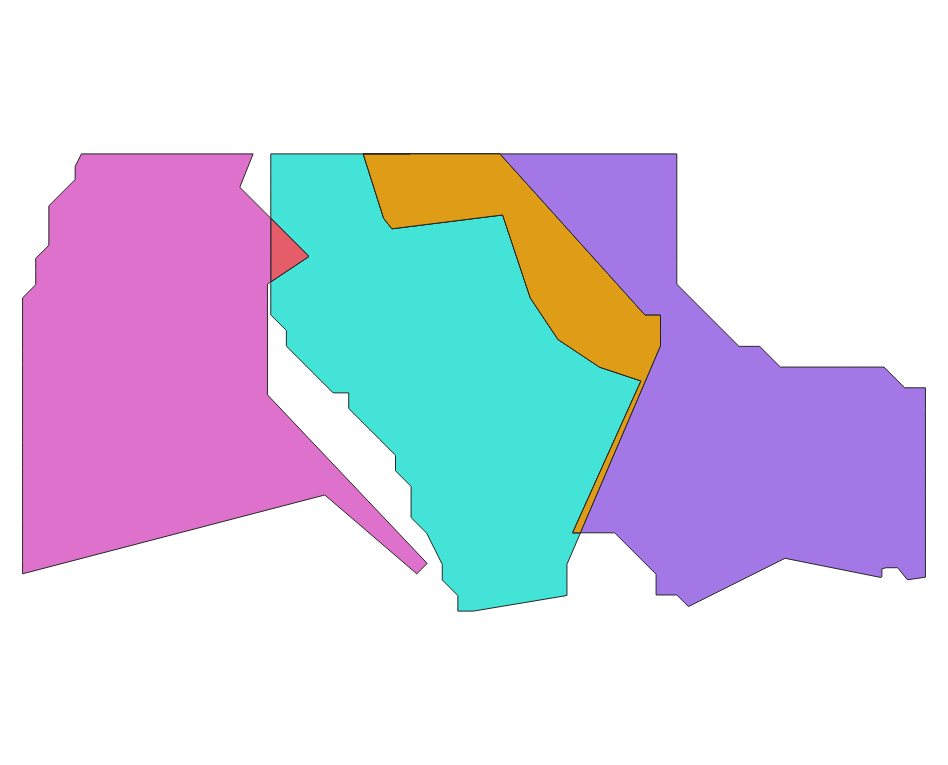
\includegraphics[width=0.60\linewidth]
        {img/sample_deter_subareas.png}
        \caption{From 3 DETER warnings, we get 7 subareas!}
        \label{fig:deter_subareas}
    \end{figure}
\end{frame}


\section{DETER subareas EDA}


\begin{frame}
    \frametitle{DETER subareas}
    \begin{figure}[h] 
        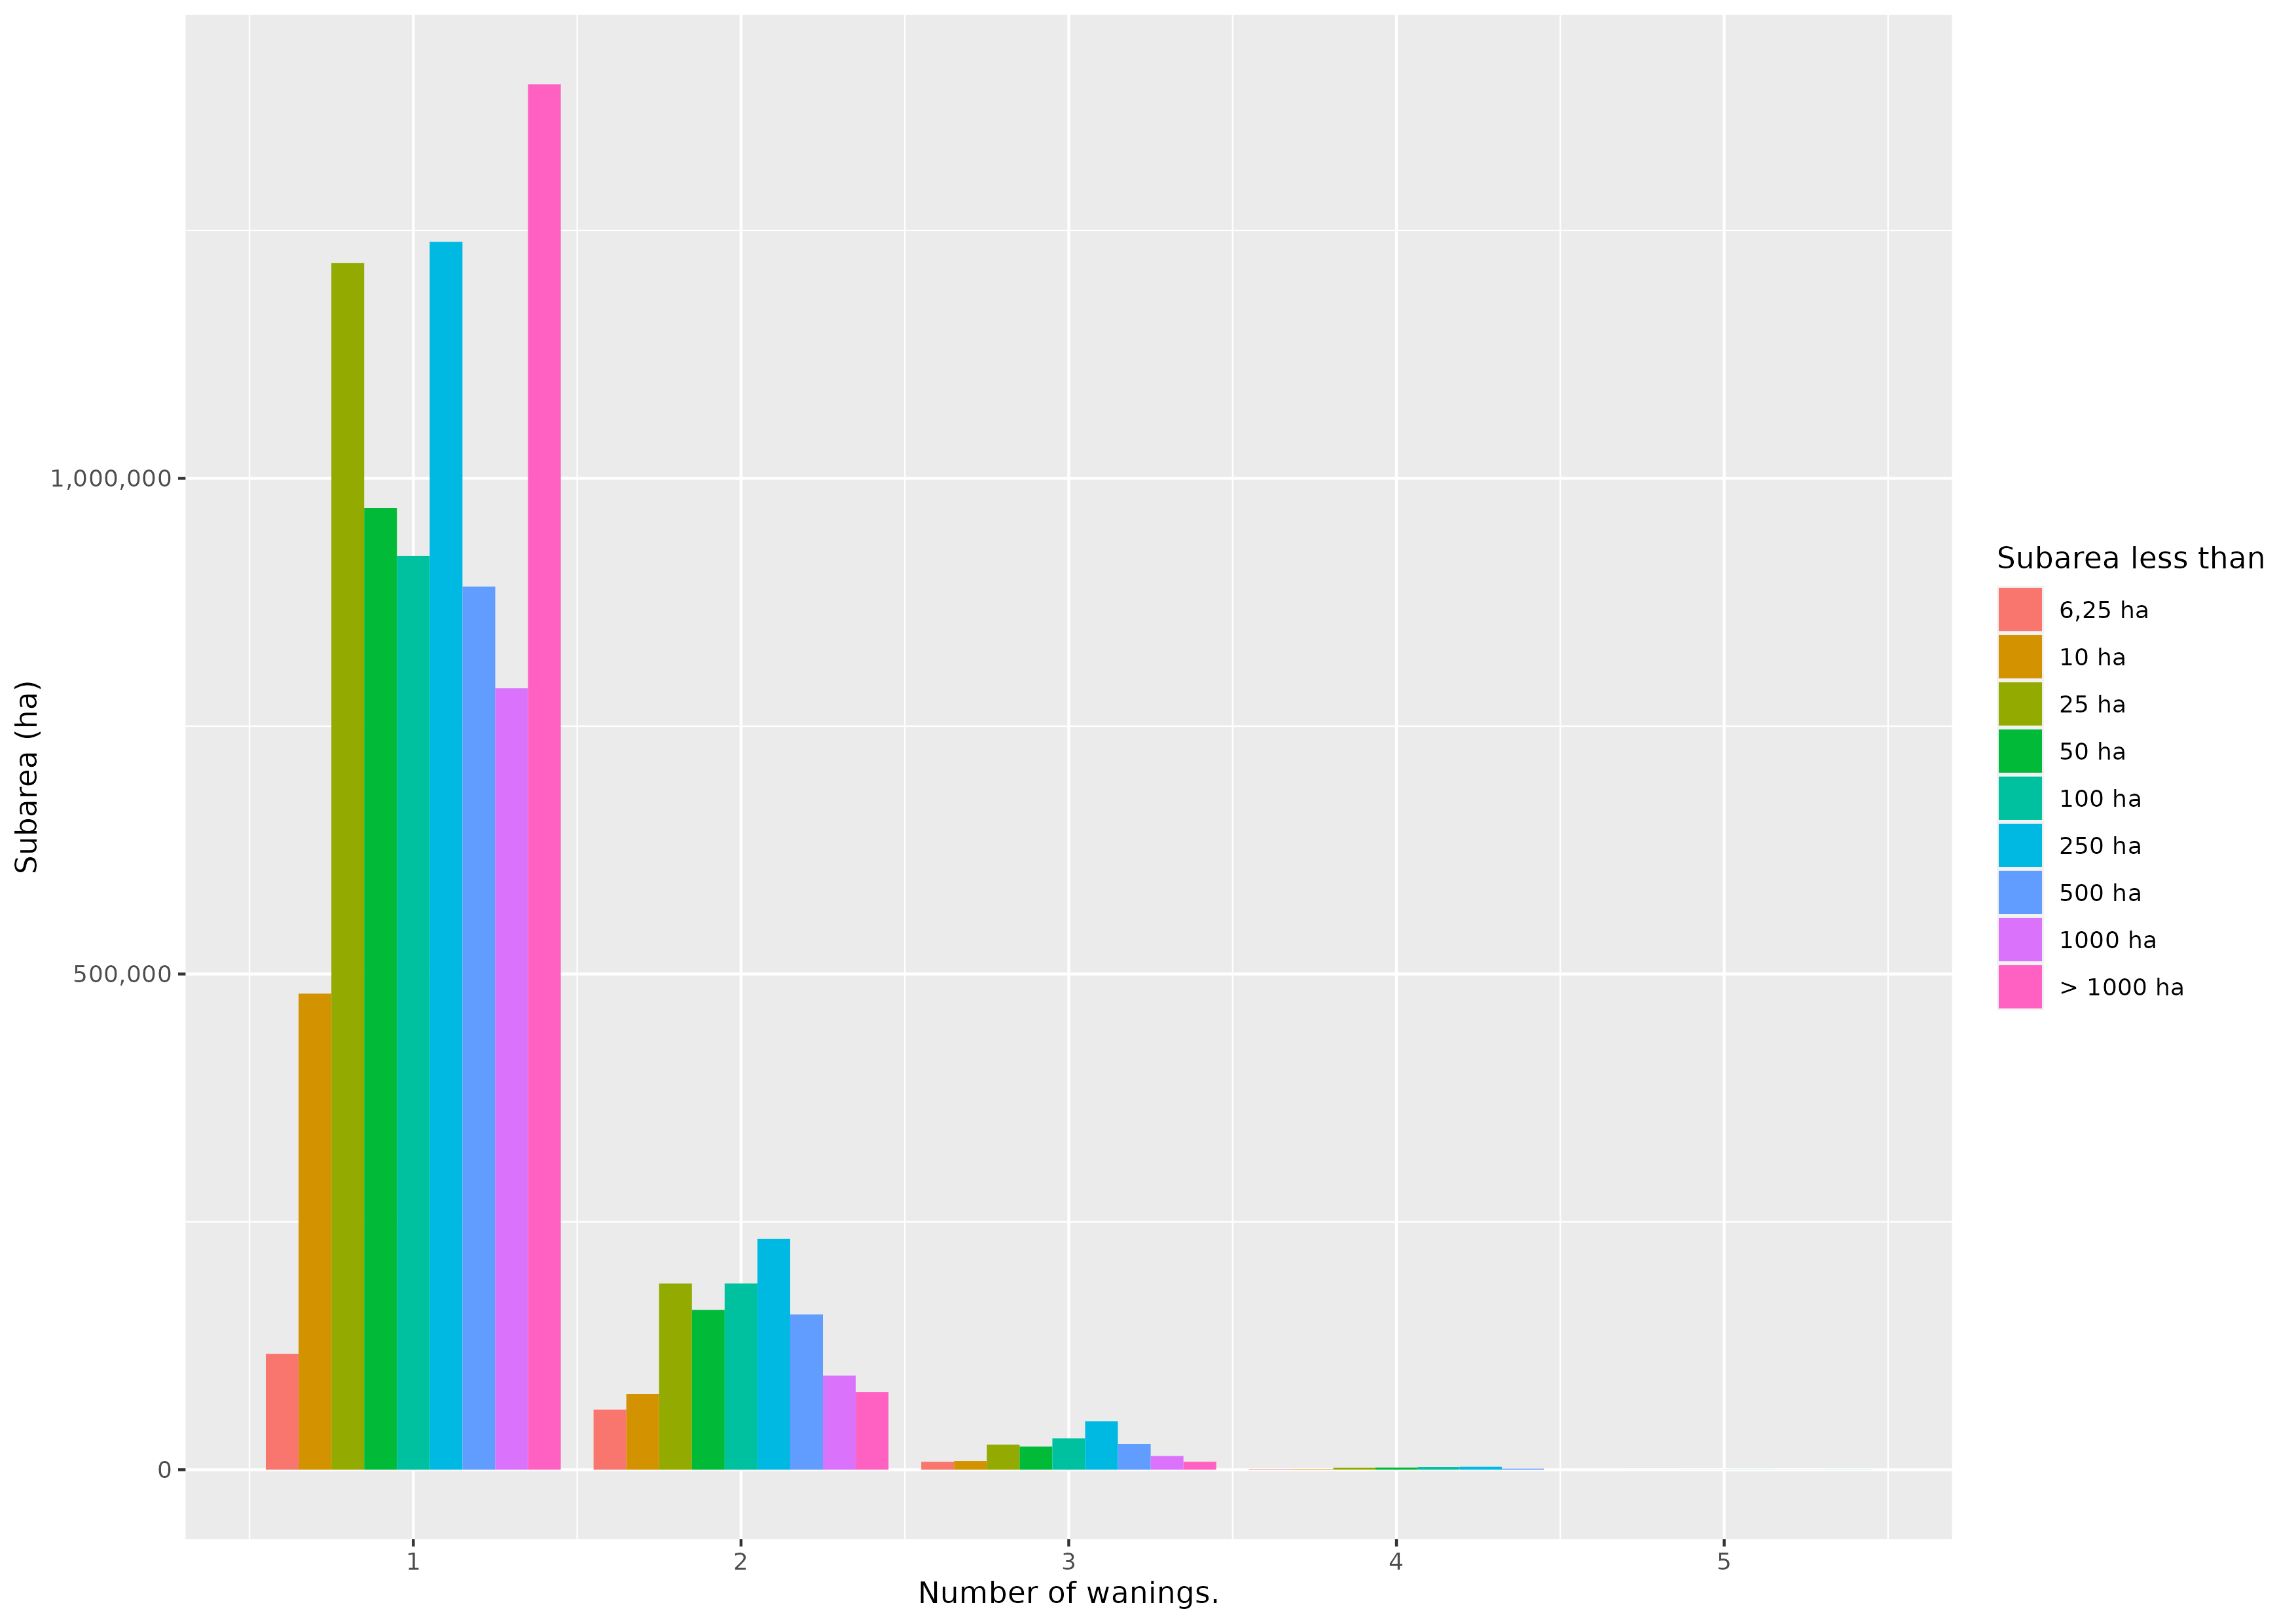
\includegraphics[width=0.7\linewidth]
        {./figures/plot_deter_subarea_by_nwarnings.png}
        \caption{There are subareas with up to 5 recurrent warnings.}
        \label{fig:deter_subareas_nwarnings}
    \end{figure}
\end{frame}

\begin{frame}
    \frametitle{DETER subareas}
    \begin{figure}[h] 
        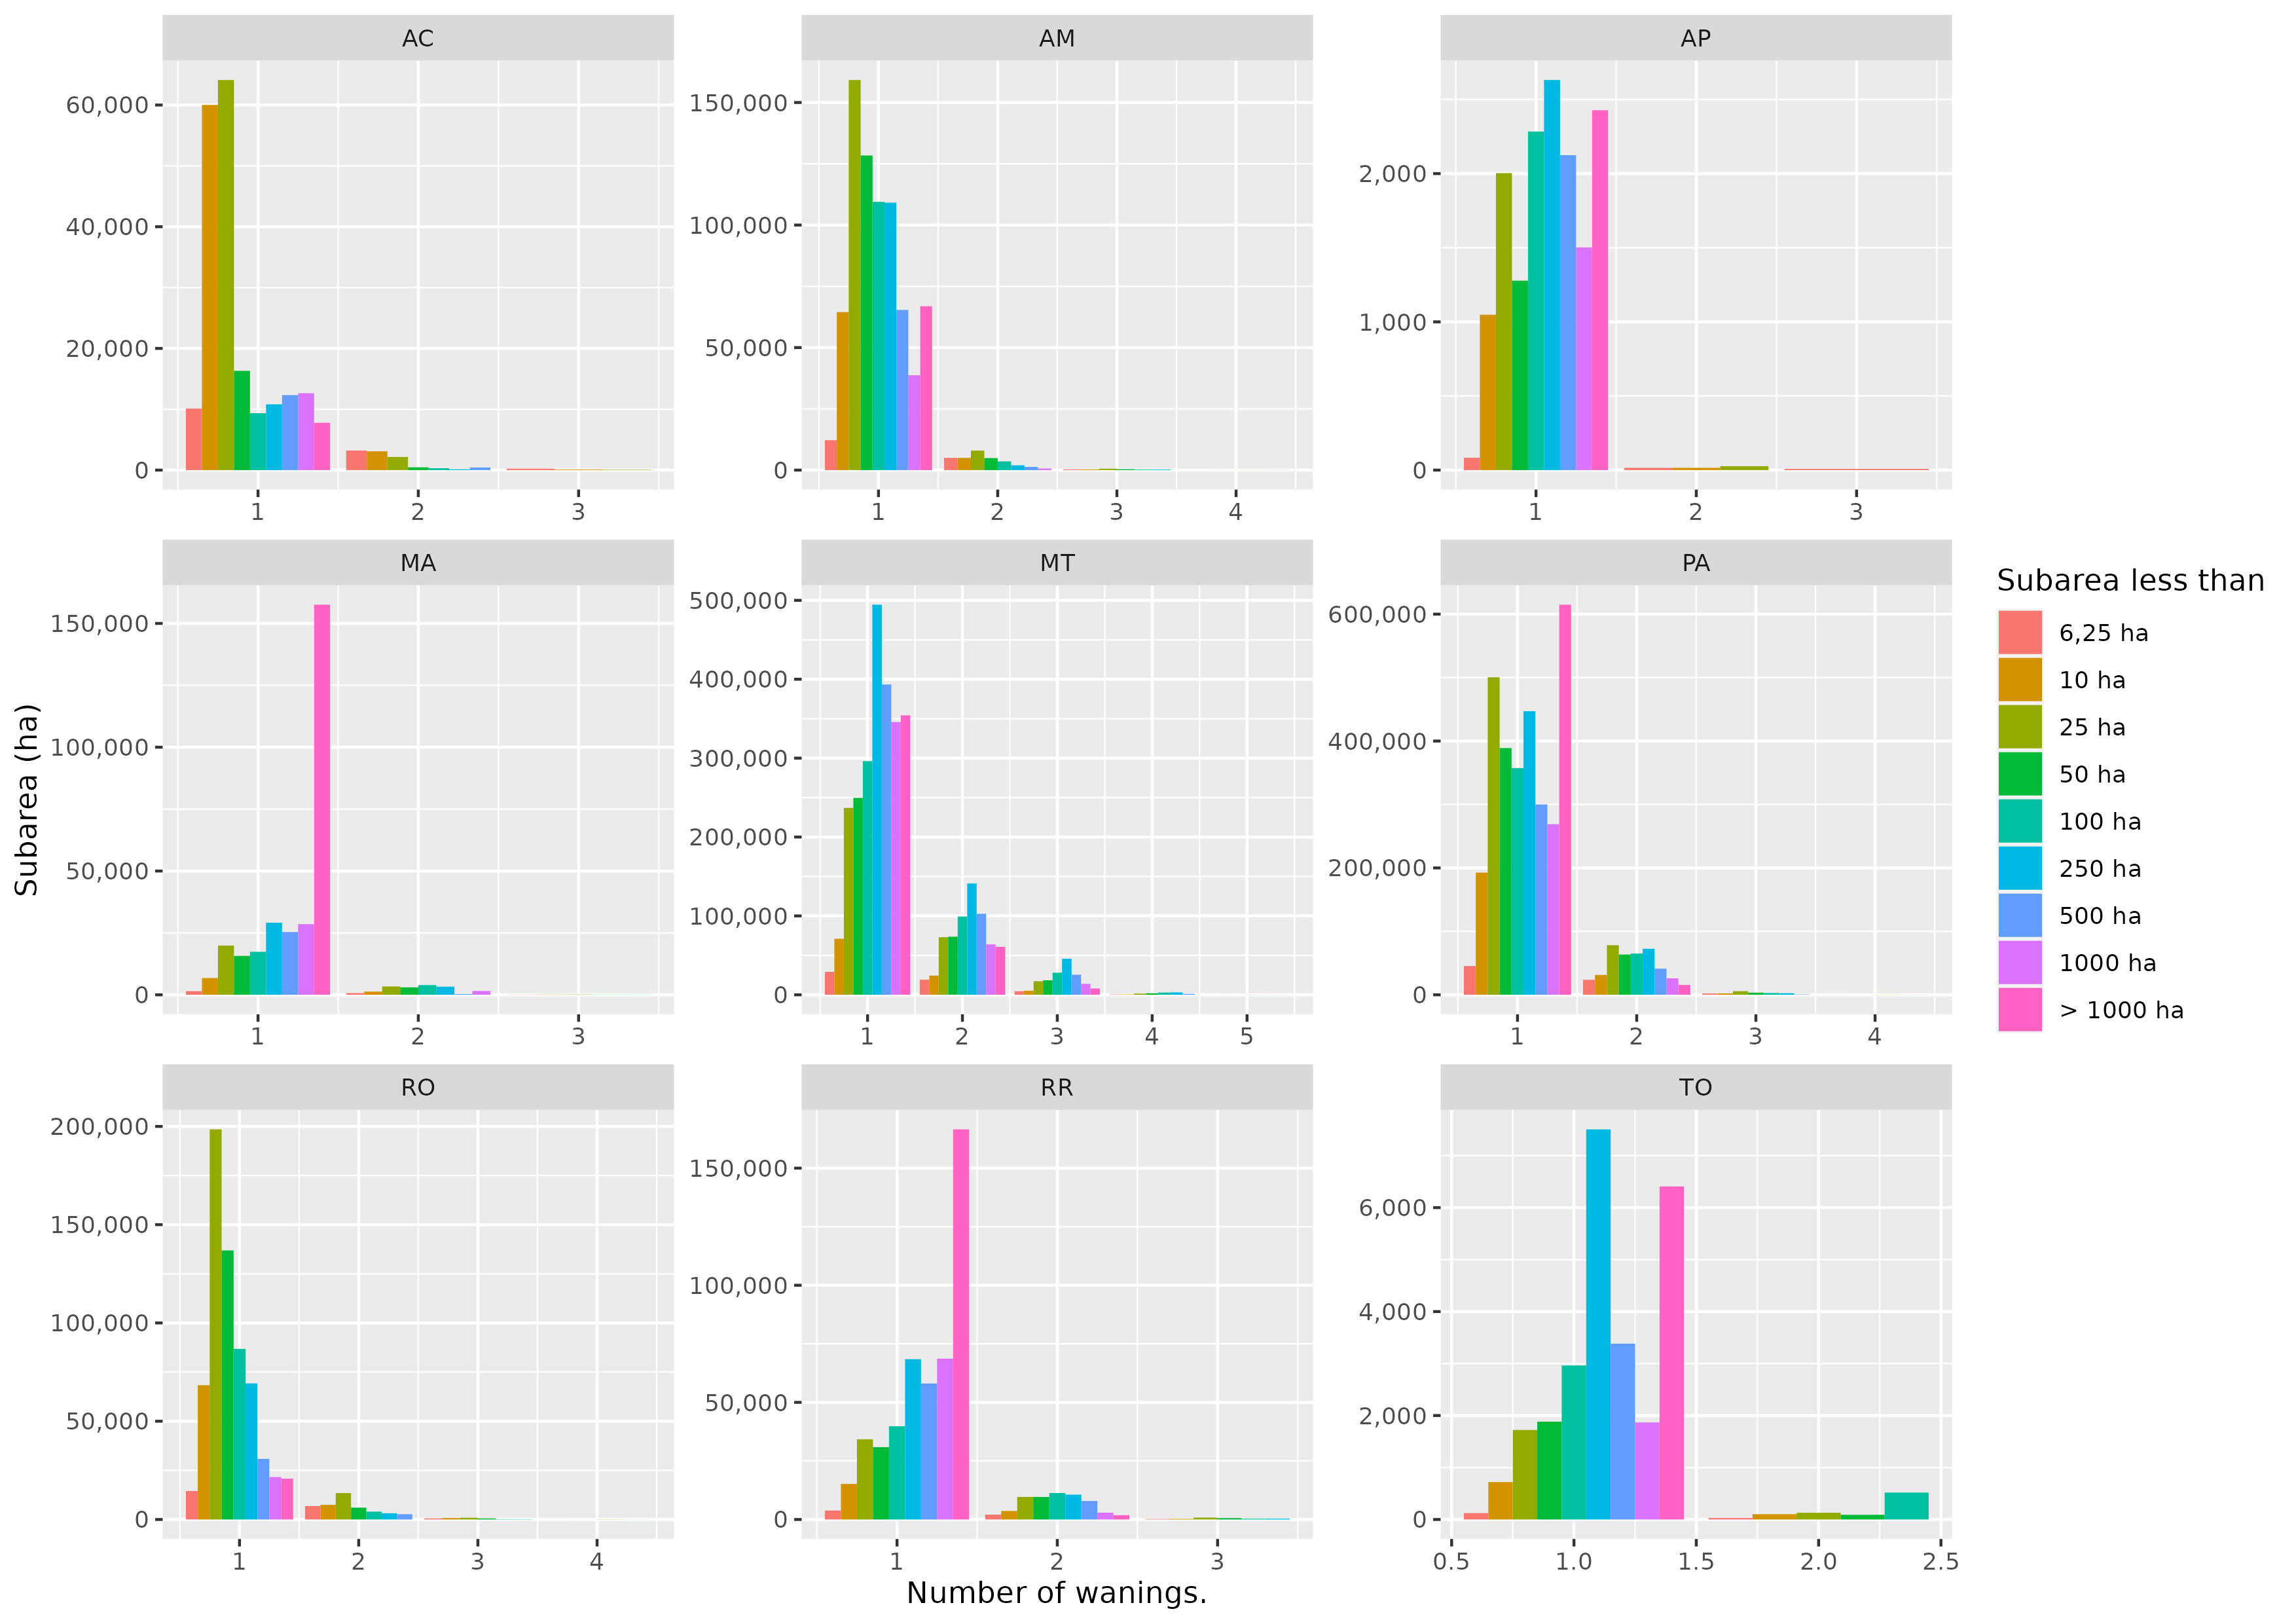
\includegraphics[width=0.65\linewidth]
        {./figures/plot_deter_subarea_by_warnings_state.png}
        \caption{The warning recurrence changes by brazilian state.}
        \label{fig:deter_subarea_warnings_state}
    \end{figure}
\end{frame}

\begin{frame}
    \frametitle{DETER subareas}
    \begin{figure}[h] 
        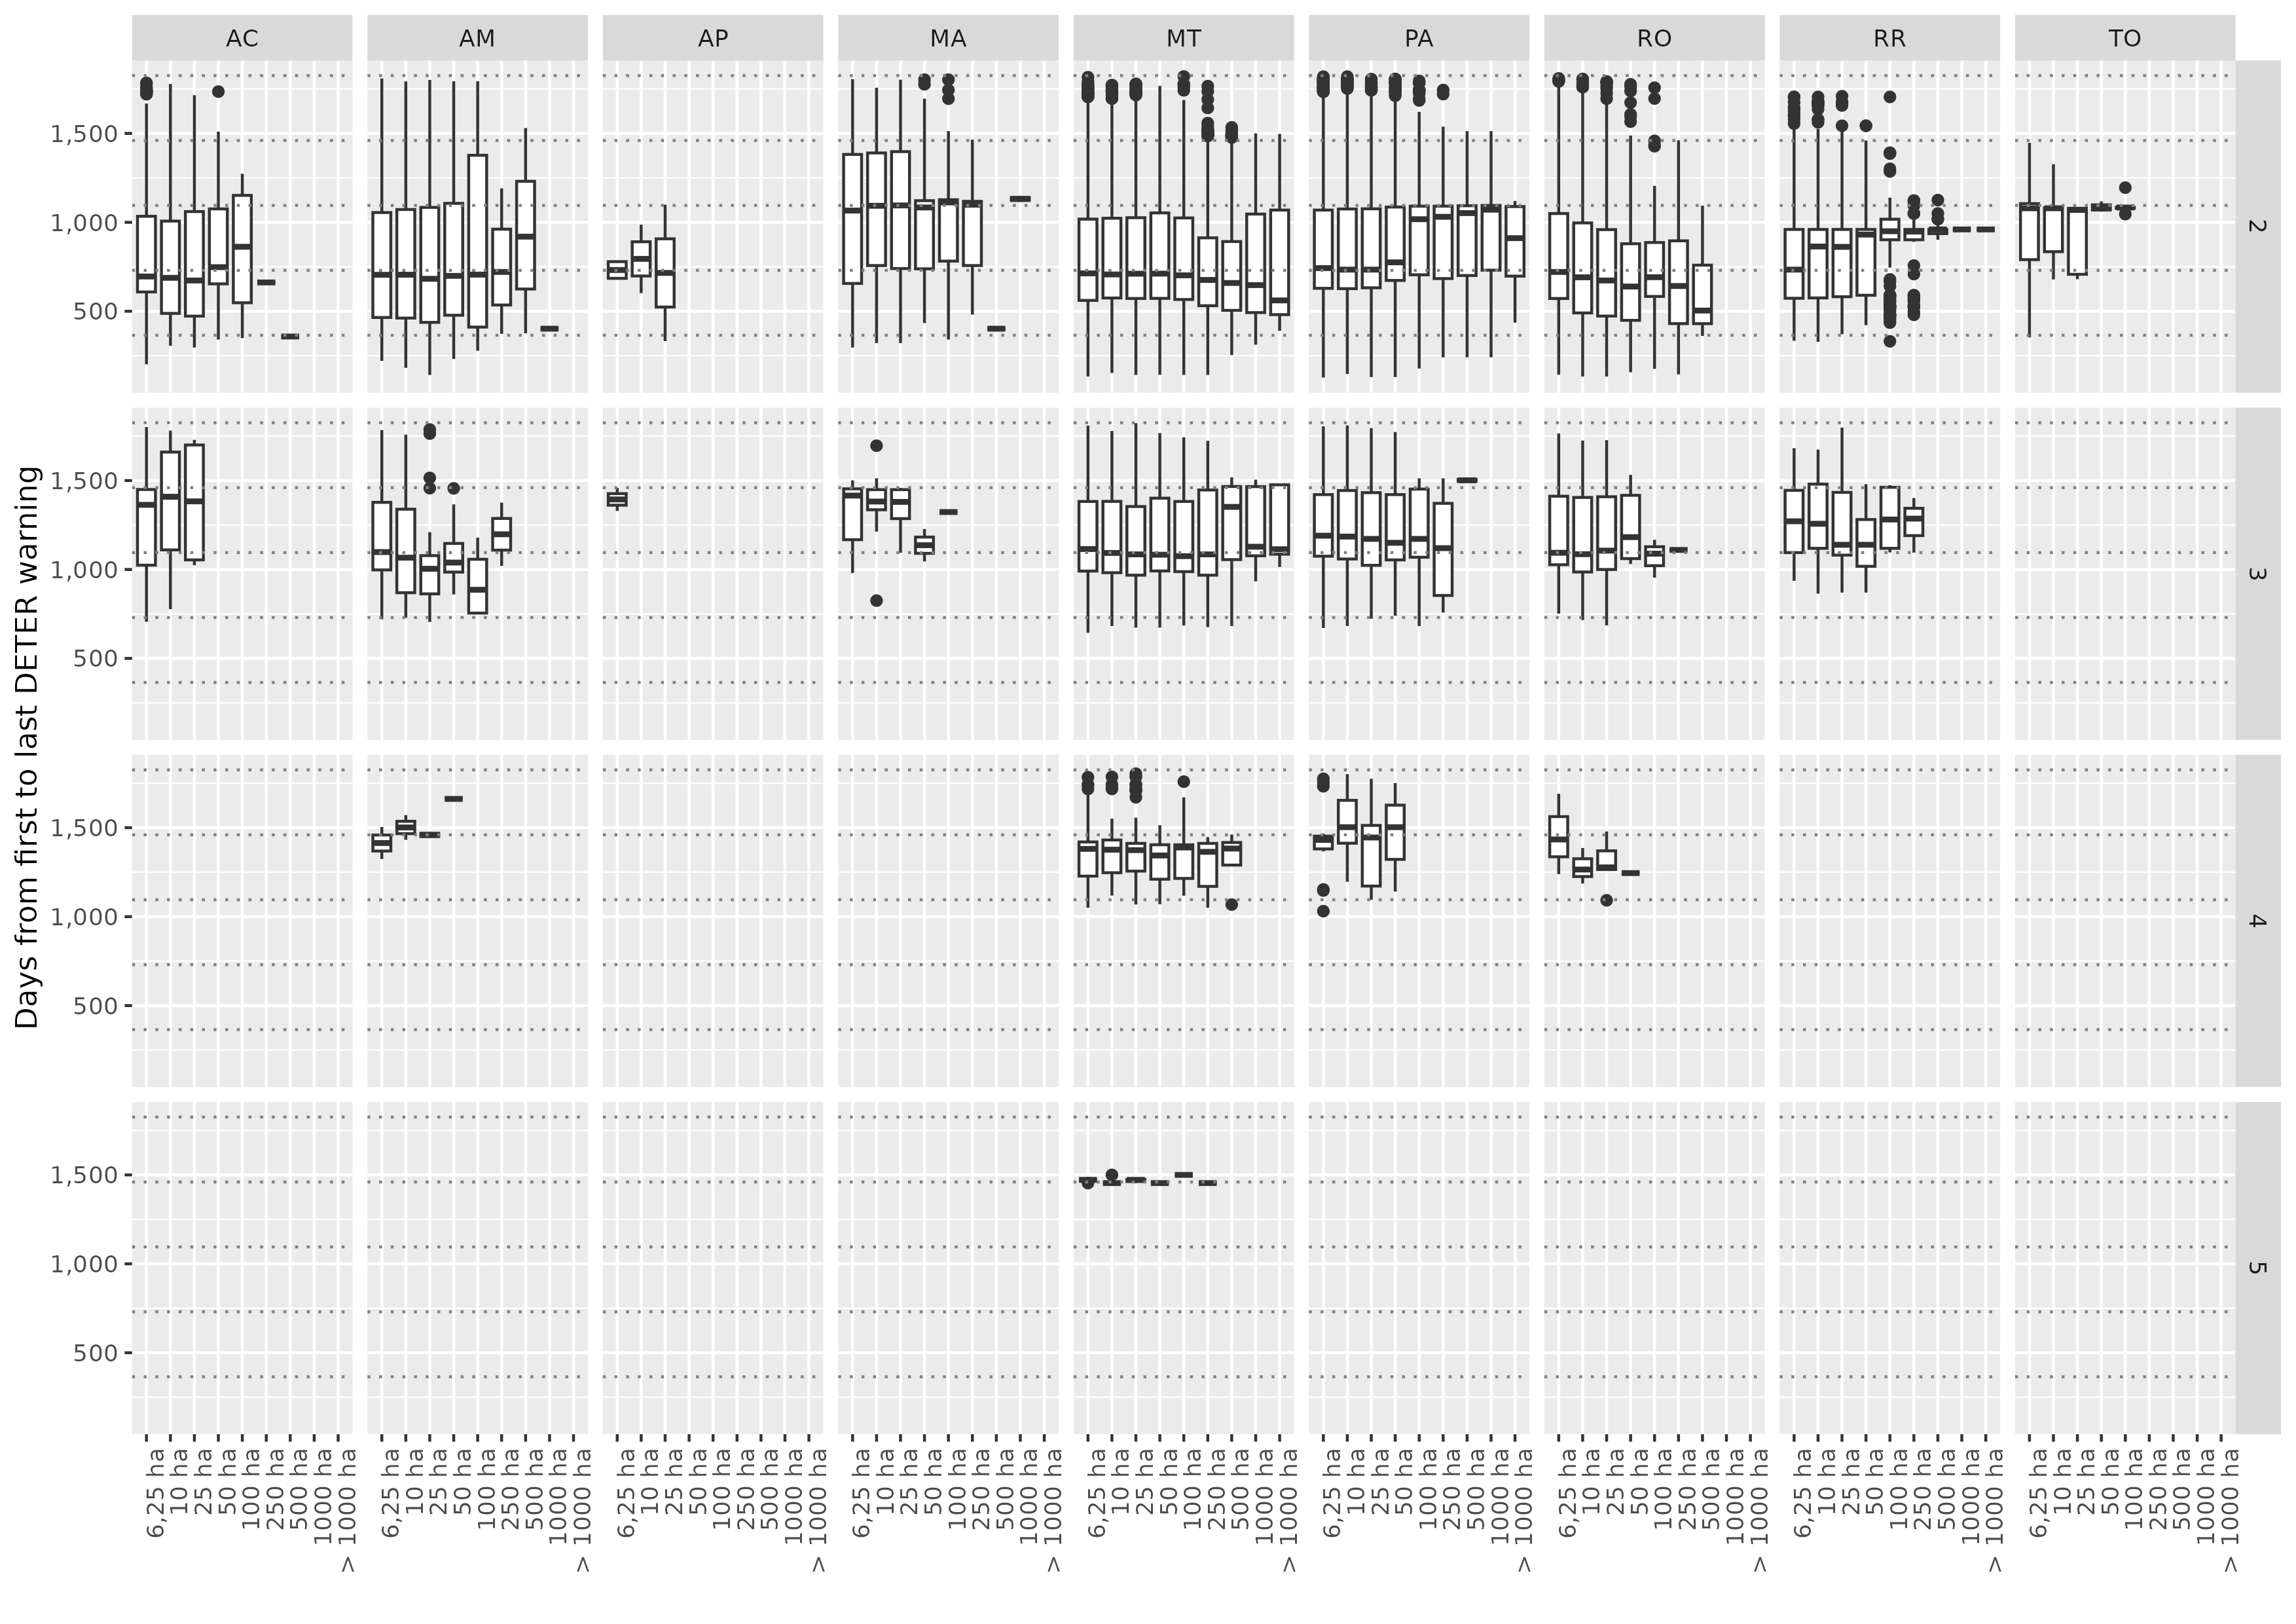
\includegraphics[width=0.7\linewidth]
        {./figures/plot_deter_days_first_to_last.png}
        \caption{Number of days between first and last warning.}
        \label{fig:deter_days_first_to_last}
    \end{figure}
\end{frame}

\begin{frame}
    \frametitle{DETER subareas}
    \begin{figure}[h] 
        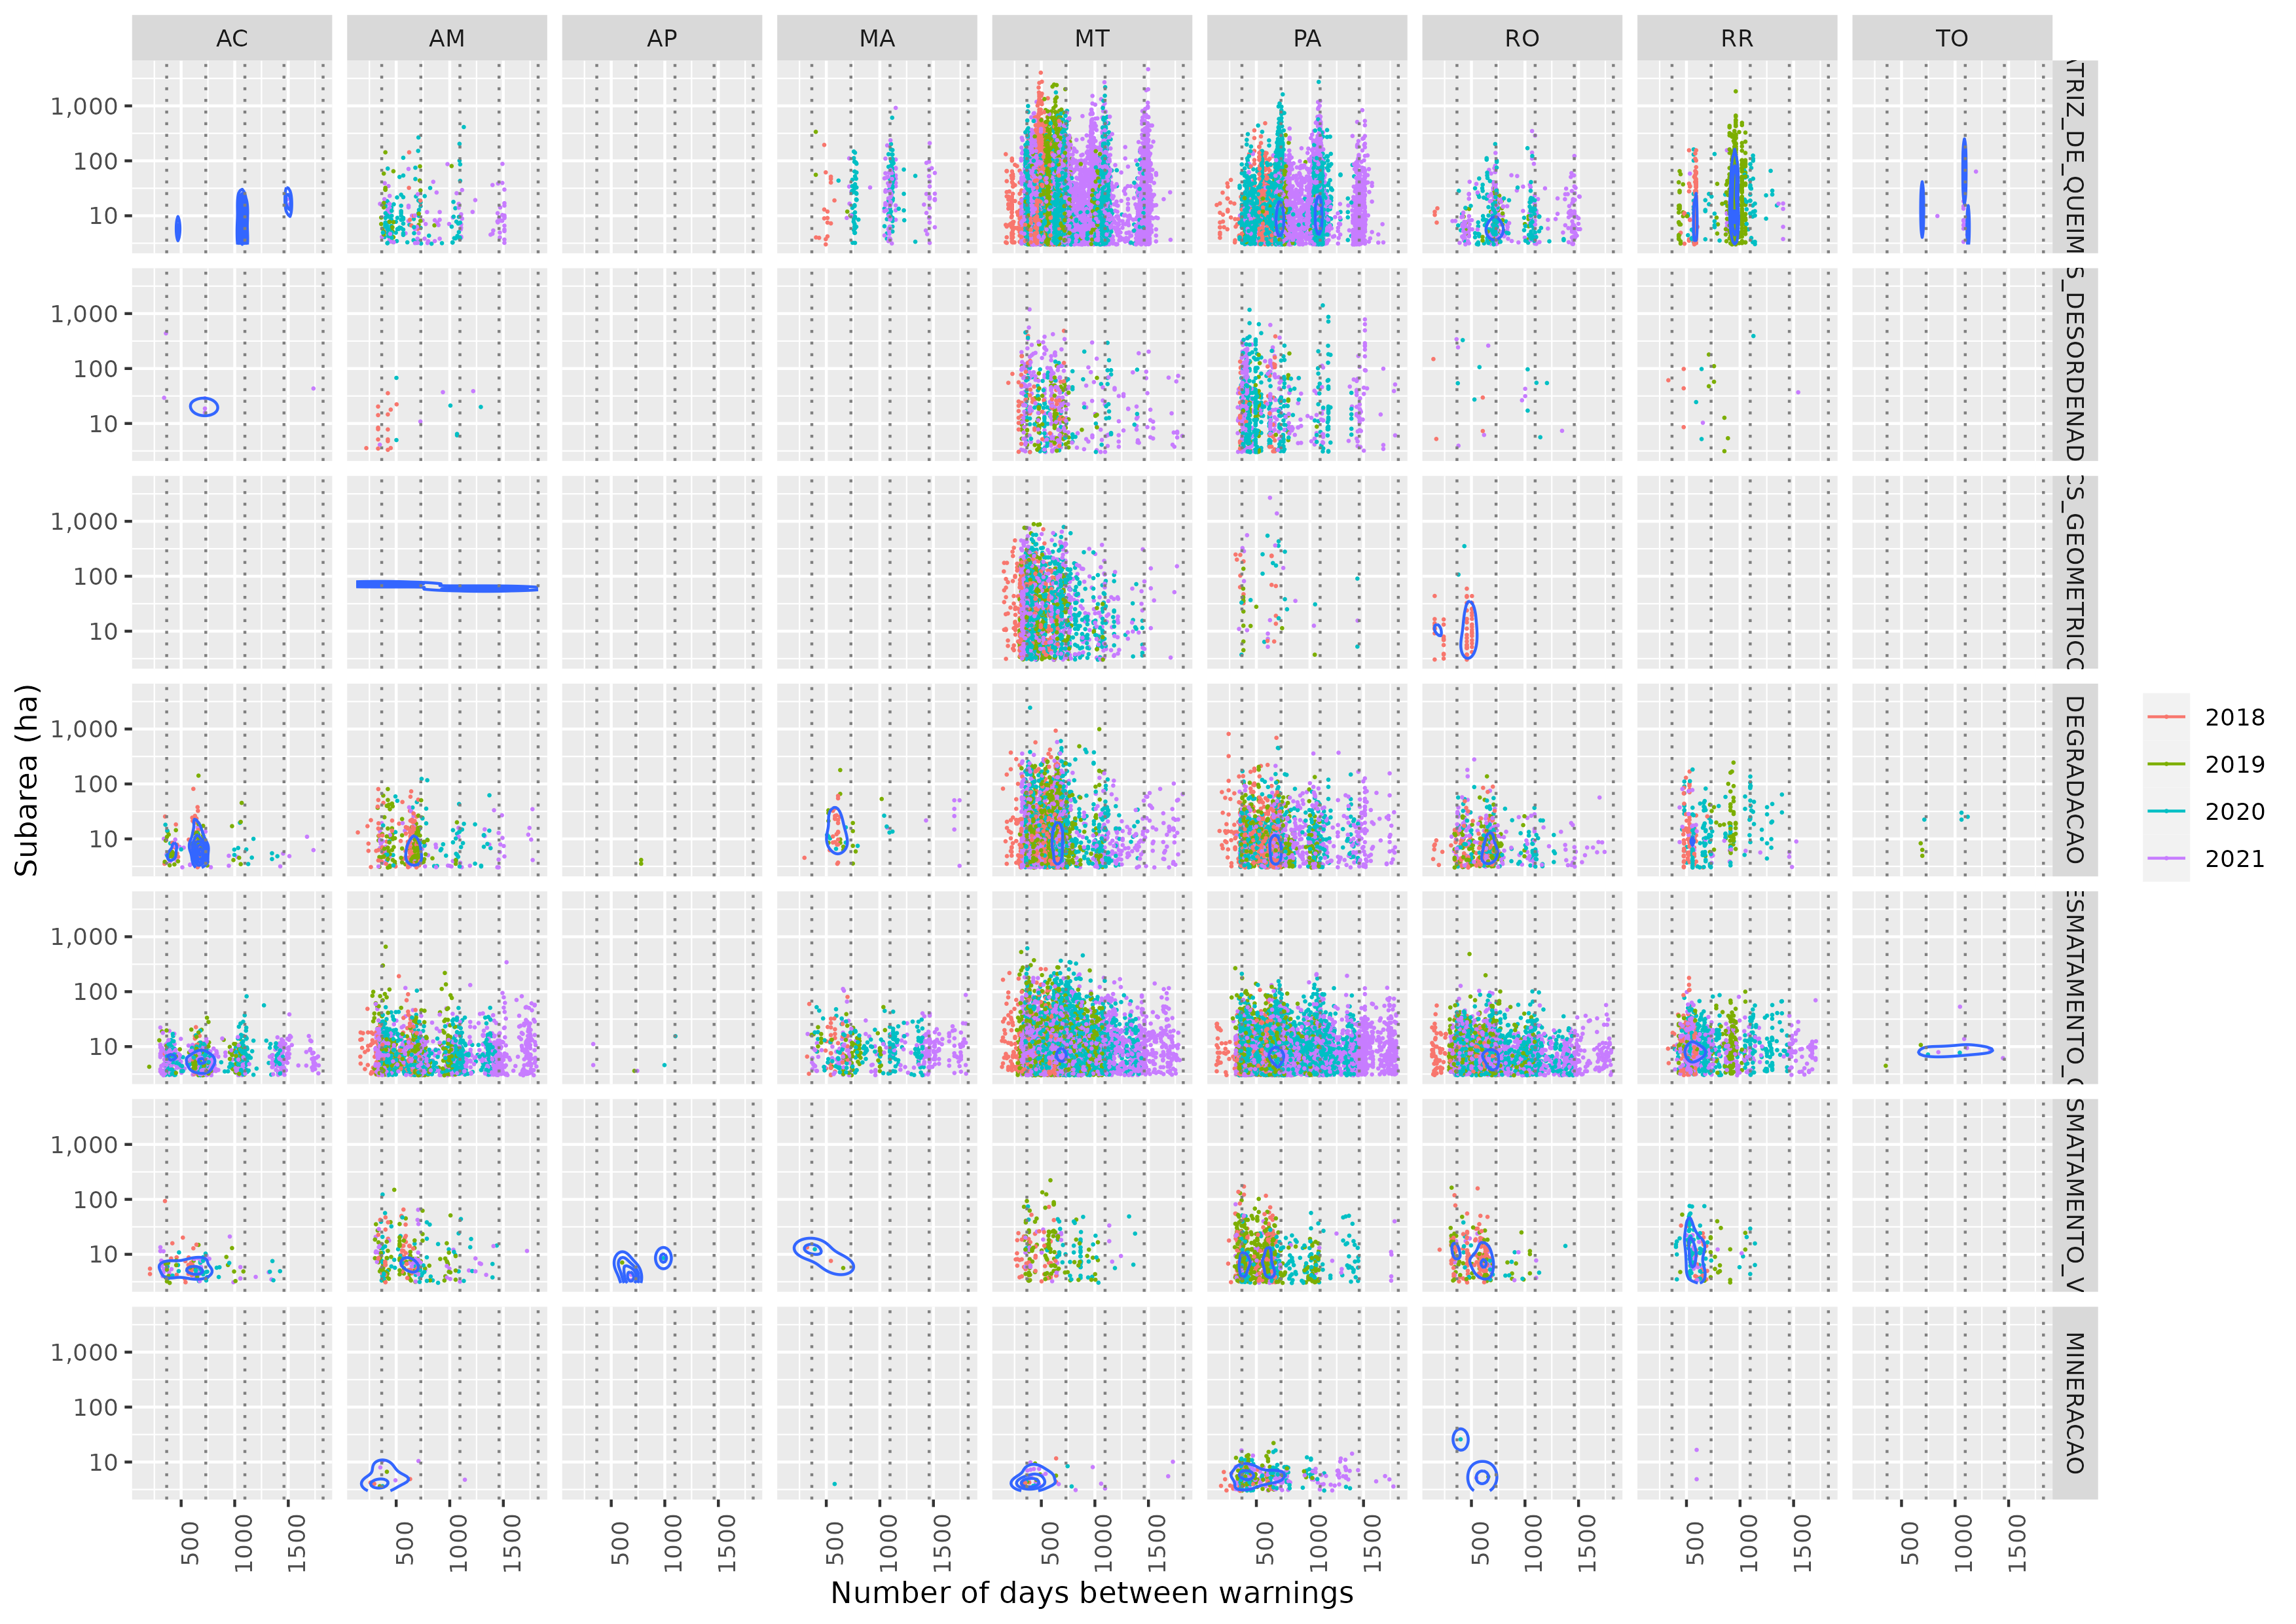
\includegraphics[width=0.65\linewidth]
        {./figures/plot_deter_subarea_density_by_state_first-type_nwarnings.png}
        \caption{The number of days between warnings behavious in space and 
        time.}
        \label{fig:deter_subarea_density_state_first_type_nwarnings}
    \end{figure}
\end{frame}


\section{Subareas trajectories} 


\begin{frame}
    \frametitle{Subarea trajectories}
    \begin{itemize}
        \item Overlaped subareas organized along time describe trajectories of
            change.
    \end{itemize}
\end{frame}


\subsection{Trajectories (DETER)} 


% \begin{frame}
%     \frametitle{DETER subareas}
%     \begin{figure}[h] 
%         \includegraphics[width=0.65\linewidth]
%         {./figures/plot_deter_subarea_trajectory_year.png}
%         \caption{Tajectory of subareas along the years.}
%         \label{fig:deter_subarea_trajectory_year}
%     \end{figure}
% \end{frame}

% \begin{frame}
%     \frametitle{DETER subareas (2 warnings)}
%     \begin{figure}[h] 
%         \includegraphics[width=0.65\linewidth]
%         {./figures/plot_deter_subarea_trajectory_2.png}
%         \caption{Tajectory of subareas with 2 wanings.}
%         \label{fig:deter_subarea_trajectory_2}
%     \end{figure}
% \end{frame}

% \begin{frame}
%     \frametitle{DETER subareas (3 warnings)}
%     \begin{figure}[h] 
%         \includegraphics[width=0.65\linewidth]
%         {./figures/plot_deter_subarea_trajectory_3.png}
%         \caption{Tajectory of subareas with 3 wanings.}
%         \label{fig:deter_subarea_trajectory_3}
%     \end{figure}
% \end{frame}

\begin{frame}
    \frametitle{DETER subareas (4 warnings)}
    \begin{figure}[h] 
        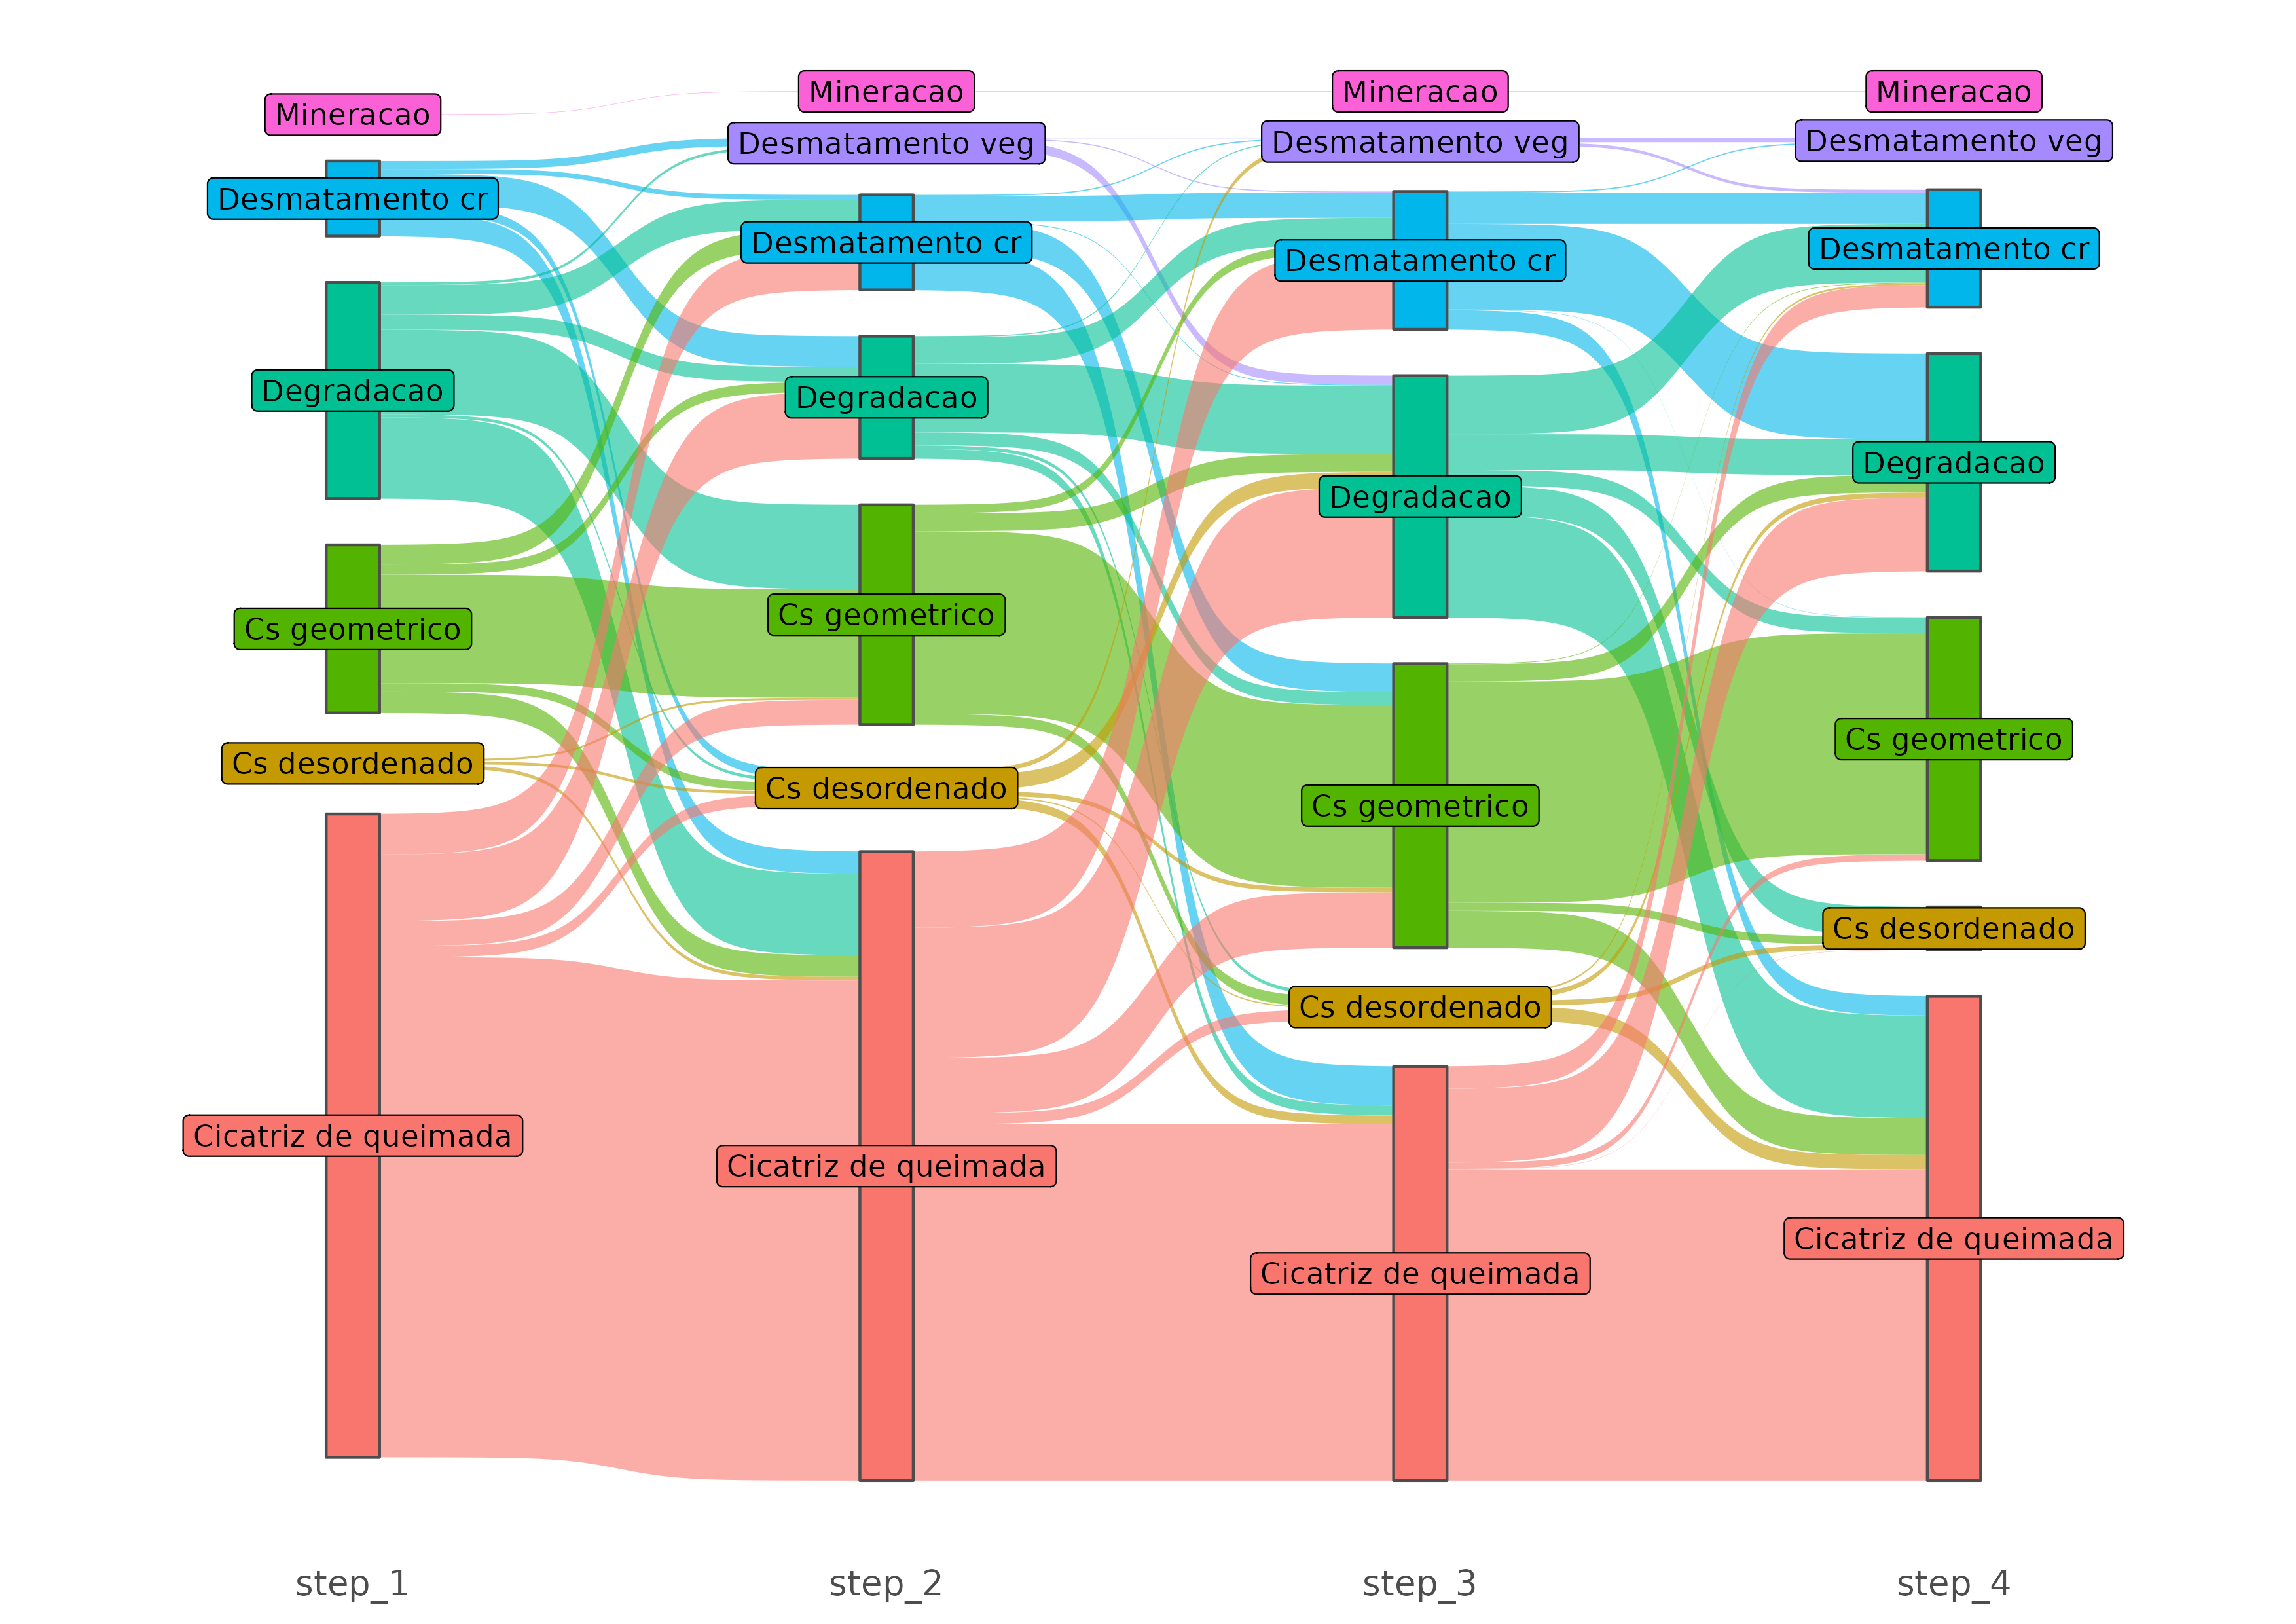
\includegraphics[width=0.65\linewidth]
        {./figures/plot_deter_subarea_trajectory_4.png}
        \caption{Tajectory of subareas with 4 wanings.}
        \label{fig:deter_subarea_trajectory_4}
    \end{figure}
\end{frame}

% \begin{frame}
%     \frametitle{DETER subareas (5 warnings)}
%     \begin{figure}[h] 
%         \includegraphics[width=0.65\linewidth]
%         {./figures/plot_deter_subarea_trajectory_5.png}
%         \caption{Tajectory of subareas with 5 wanings.}
%         \label{fig:deter_subarea_trajectory_5}
%     \end{figure}
% \end{frame}


% \subsection{Trajectories (DETER \& PRODES)} 
%
%
% \begin{frame}
%     \frametitle{DETER \& PRODES}
%     \begin{itemize}
%         \item Add to the trajectories the PRODES class corresponding to each
%             DETER subarea.
%         \item The selected class corresponds to the mode of PRODES' pixels in
%             each DETER subarea.
%         \item Use PRODES' view date to sort trajectories.
%     \end{itemize}
% \end{frame}

% \begin{frame}
%     \frametitle{DETER \& PRODES subareas (2 warnings)}
%     \begin{figure}[h] 
%         \includegraphics[width=0.65\linewidth]
%         {./figures/plot_deter_prodes_subarea_trajectory_2.png}
%         \caption{Tajectory of subareas with 2 warnings.}
%         \label{fig:deter_prodes_subarea_trajectory_2}
%     \end{figure}
% \end{frame}

% \begin{frame}
%     \frametitle{DETER \& PRODES subareas (3 warnings)}
%     \begin{figure}[h] 
%         \includegraphics[width=0.65\linewidth]
%         {./figures/plot_deter_prodes_subarea_trajectory_3.png}
%         \caption{Tajectory of subareas with 3 wanings.}
%         \label{fig:deter_prodes_subarea_trajectory_3}
%     \end{figure}
% \end{frame}

% \begin{frame}
%     \frametitle{DETER \& PRODES subareas (4 warnings)}
%     \begin{figure}[h] 
%         \includegraphics[width=0.65\linewidth]
%         {./figures/plot_deter_prodes_subarea_trajectory_4.png}
%         \caption{Tajectory of subareas with 4 wanings.}
%         \label{fig:deter_prodes_subarea_trajectory_4}
%     \end{figure}
% \end{frame}

% \begin{frame}
%     \frametitle{DETER \& PRODES subareas (5 warnings)}
%     \begin{figure}[h] 
%         \includegraphics[width=0.65\linewidth]
%         {./figures/plot_deter_prodes_subarea_trajectory_5.png}
%         \caption{Tajectory of subareas with 5 wanings.}
%         \label{fig:deter_prodes_subarea_trajectory_5}
%     \end{figure}
% \end{frame}

% \begin{frame}
%     \frametitle{DETER \& PRODES subareas (6 warnings)}
%     \begin{figure}[h] 
%         \includegraphics[width=0.65\linewidth]
%         {./figures/plot_deter_prodes_subarea_trajectory_6.png}
%         \caption{Tajectory of subareas with 6 wanings.}
%         \label{fig:deter_prodes_subarea_trajectory_6}
%     \end{figure}
% \end{frame}

%%%%%%%%%%%%%%%%%%%%%%%%%%%%%%%%%%%%%%%%%%%%%%%%%%%%%%%%%%%%%%%%%%%%%%%%%%%%%%%

% TODO: 
% - slides talking about fitness for use and purpose of DETER regarding Fire
% - smooth the transition from deforestation to fire
% - Cut to maximum 20 slides 

\begin{frame}
  \frametitle{Take home message}
  \begin{itemize}
    \item Deforestation and forest degradation threat the Amazon.
    \item An important portion of deforestation and degradation are due to 
      fire.
    \item We need to take advantage of all available resources and search for 
      answers to the urgent questions post by a fast changing climate.
     \item The analysis of DETER warnings could improve the characterization 
       of forest degradation just by switching to a perspective that focus 
       on the time dimension instead of the spatial dimensions.
     \item R code available at 
         \url{https://github.com/albhasan/treesburnareas}
  \end{itemize}
\end{frame}

\begin{frame}[allowframebreaks]
  \frametitle{References}
  \bibliographystyle{amsalpha}
  \bibliography{slides.bib}
\end{frame}

\end{document}


% \subsection{Successive degradation}


% \begin{frame}
%     \frametitle{Deforestation by successive degradation}
%     \begin{itemize}
%         \item Deforestation by successive degradation remains a challenging 
%             question in the scientific literature.
%         \item We think an answer to this question lies down in DETER data.
%         \item This answer could play an important role, for example, in the 
%             brazilian estimation of greenhouse gases.
%         \item We used DETER data from 2016 to 2021 of the Amazon Biome in 
%               Brazil.
%     \end{itemize}
% \end{frame}


% \subsection{DETER}





% \subsection{Analysis 1}


% \begin{frame}
%     \frametitle{Analysis 1}
%     \begin{itemize}
%         \item Trajectories have one event in each PRODES year. There were 
%             70/517059 with more than one.
%         \item Trajectories related to mining were excluded.
%         \item Trajectories end as soon as they reach deforestation.
%         \item Trajectories include at least one PRODES event.
%     \end{itemize}
% \end{frame}
%
% \begin{frame}
%   \frametitle{Analysis 1 (2 warnings) }
%   \begin{figure}[h] 
%   \includegraphics[width=0.65\textwidth]
%     {figures/an1_plot_deter_prodes_subarea_trajectory_2.png}
%   \end{figure}
% \end{frame}
%
% \begin{frame}
%     \frametitle{Analysis 1 (3 warnings) }
%     \begin{figure}[h] 
%     \includegraphics[width=0.65\textwidth]
%       {figures/an1_plot_deter_prodes_subarea_trajectory_3.png}
%     \end{figure}
% \end{frame}
%
% \begin{frame}
%     \frametitle{Analysis 1 (4 warnings) }
%     \begin{figure}[h] 
%     \includegraphics[width=0.65\textwidth]
%       {./figures/an1_plot_deter_prodes_subarea_trajectory_4.png}
%     \end{figure}
% \end{frame}
%
% \begin{frame}
%     \frametitle{Analysis 1 (5 warnings) }
%     \begin{figure}[h] 
%     \includegraphics[width=0.65\textwidth]
%       {./figures/an1_plot_deter_prodes_subarea_trajectory_5.png}
%     \end{figure}
% \end{frame}
%
%
% \subsection{Analysis 2}
%
%
% \begin{frame}
%     \frametitle{Analysis 2}
%     \begin{itemize}
%         \item Same as Analysis 1, but only using DETER's burn scars.
%     \end{itemize}
% \end{frame}
%
% \begin{frame}
%     \frametitle{Analysis 2 (2 warnings) }
%     \begin{figure}[h] 
%     \includegraphics[width=0.65\textwidth]
%       {./figures/an2_plot_deter_prodes_subarea_trajectory_2.png}
%     \end{figure}
% \end{frame}
%
% \begin{frame}
%     \frametitle{Analysis 2 (3 warnings) }
%     \begin{figure}[h] 
%     \includegraphics[width=0.65\textwidth]
%       {./figures/an2_plot_deter_prodes_subarea_trajectory_3.png}
%     \end{figure}
% \end{frame}
%
% \begin{frame}
%     \frametitle{Analysis 2 (4 warnings) }
%     \begin{figure}[h] 
%     \includegraphics[width=0.65\textwidth]
%       {./figures/an2_plot_deter_prodes_subarea_trajectory_4.png}
%     \end{figure}
% \end{frame}
%
% \begin{frame}
%     \frametitle{Analysis 2 (5 warnings) }
%     \begin{figure}[h] 
%     \includegraphics[width=0.65\textwidth]
%       {./figures/an2_plot_deter_prodes_subarea_trajectory_5.png}
%     \end{figure}
% \end{frame}


% \section{Fire spots}


% \begin{frame}
%     \frametitle{Fire spots}
%     \begin{itemize}
%         \item We downloaded fire spots from INPE's \emph{Queimadas} project.
%         \item The data corresponds to VIIRS satellite (NPP-375 morning and 
%             afternoon).
%     \end{itemize}
% \end{frame}

% \begin{frame}
%     \frametitle{Current analysis venue}
%     \begin{itemize}
%         \item How to convert fires spots into fire events?
%         \item For example, ~\cite{andela2022} had the same problem.
%         \item DETER data contrains the problem's spatial domain.
%     \end{itemize}
% \end{frame}


% % \section{Closing}

% % \begin{frame}
% %     \frametitle{Final remarks}
% %     \begin{itemize}
% %         \item The analysis of DETER warning subareas along time could improve 
% %             the characterization of forest degradation along time.
% %         \item Potential applications of our work are:
% %             \begin{itemize}
% %                 \item Improve estimation of emissions of greenhouse gases, i.e.
% %                     our data could help avoiding double counting.
% %                 \item Identify spatio-temporal areas which could help training 
% %                     Machine-Learning algorithms for automatic indentification 
% %                     of forest degradation.
% %             \end{itemize}
% %         \item Code available at 
% %             \url{https://github.com/albhasan/treesburnareas}
% %     \end{itemize}
% % \end{frame}

% \begin{frame}
%   \frametitle{Plano Amazônia}
%   \begin{columns}
%     \begin{column}{0.4\textwidth}
%       \begin{itemize}
%         \item Plano Amazônia 2021\slash2022 prioritizes law enforcement in 11 
%           municipalities.
%         \item Maximize success by focusing law enforcement on small areas with 
%           the highest deforestation.
%       \end{itemize}
%       However, 
%       \begin{itemize}
%         \item Environmental institutes (such as IBAMA and ICMBio) have been 
%           suffering massive budget cuts.
%         \item Leakage of law enforcement actions are causing new deforestation 
%           hotspots.
%       \end{itemize}
%     \end{column}
%     \begin{column}{0.6\textwidth}
%       \begin{figure}
%         \centering
%         \includegraphics[width=0.9\textwidth]
%         {img/pa2021_priorized_towns.png}
%         \caption{Prioritized municipalities by PA\slash21\slash22. 
%         Source~\cite{mataveli2022}.}
%         \label{fig:prioritized_towns_pa}
%       \end{figure}
%     \end{column}
%   \end{columns}
% \end{frame}

% \begin{frame}[allowframebreaks]
%     \frametitle{DETER \& PRODES - proximity in time}
%     \begin{itemize}
%         \item There is a potential DETER-PRODES overlap in our analysis.
%         \item DETER warnings and PRODES deforestation polygons could refer to
%             the same event.
%         \item The next slide reports the DETER warnings closest in 
%             time to PRODES polygons.
%     \end{itemize}
% \end{frame}



